% Nejprve uvedeme tridu dokumentu s volbami
\documentclass[czech,master,public,dept460,male,cpdeclaration]{diploma}	% jednostranny dokument

\usepackage[utf8]{inputenc}
\inputencoding{utf8}
\usepackage[czech]{babel}

\usepackage{subfig}		% makra pro "podobrazky" a "podtabulky"
\usepackage{tikz}		% makra pro kresleni

\usepackage{makecell}

\usepackage{pdflscape}

\usepackage{placeins}


\newcommand{\iic}{I\textsuperscript{2}C }
\newcommand{\iis}{I\textsuperscript{2}S }
\newcommand{\eeprom}{E\textsuperscript{2}PROM}

\newcommand{\VID}{0x04D8}
\newcommand{\PID}{0xF32C}

%\widowpenalty10000
%\clubpenalty10000


% Zadame pozadovane vstupy pro generovani titulnich stran.
\ThesisAuthor{Bc. Pavel Kovář}

% U bakalarske praxe neni nutne nazev zadavat
\CzechThesisTitle{Modul USB FM rádia}

% U bakalarske praxe neni nutne anglicky nazev zadavat
\EnglishThesisTitle{USB FM Radio Modul}

\SubmissionDate{27. dubna 2016}

%\PrintPublicationAgreement{true}

\Thanks{Rád bych na tomto místě poděkoval mému vedoucímu panu Ing. Davidu Seidlovi, Ph.D. za cenné rady a trpělivost.}

\CzechAbstract{Tato práce popisuje návrh USB FM přijímače se dvěma tunery. Jeden tuner slouží pro přehrávání zvuku a~druhý pro vyhledávání dalších stanic. přijímač je v~systému reprezentován jako USB zvuková karta.\\ 
Příjem je realizován dvojicí integrovaných obvodů Si4735-DU. Tyto jsou přes \iis a \iic  spojeny s~MCU PIC32MX250F128B, který přes USB zajišťuje komunikaci s počítačem. V rámci firmware MCU je, po neúspěchu s Microchip harmony frameworkem, napsán vlastní USB stack.\\
Knihovna je napsána v jazyku~C s~využitím knihovny libusb. Poskytuje funkce pro tři úrovně přístupu k~tunerům.\\
Demonstrační aplikace je ve formě grafického uživatelského rozhraní, napsaná  v~C++ s využitím QT frameworku.\\
Vše je funkční pod OS Linux i~Windows.}

\CzechKeywords{FM rádio, USB, RDS, QT, libusb, PIC}

\EnglishAbstract{This work describes design of USB FM radio receiver with two tuners. One tuner is for radio playback, second one seeks new stations. In computer, device acts as sound card.\\
Receiving is done by couple of Si4735-DU integrated circuits, which are connected to MCU via \iic and \iis. MCU forwards data over USB to computer and back. Use of Microchip harmony framework was not successful so in firmware is USB stack written from scratch.\\
Library is written in C with use of libusb library. There are three levels of functions to access tuners.\\
Demo application has graphical user interface and is written in C++ in QT framework.\\
All works under Linux and Windows.}

\EnglishKeywords{FM radio receiver, USB, RDS, QT, libusb, PIC}

% Pridame pouzivane zkratky (pokud nejake pouzivame).
\AddAcronym{AM}{Amlitudová Modulace (Rozhlasové vysílání v pásmu dlouhých vln)}
\AddAcronym{CD}{Compact disc}
\AddAcronym{DAB}{Digital Audio Broadcasting (Digitální pozemní rozhlasové vysílání)}
\AddAcronym{DIP}{Dual Inline Package}
\AddAcronym{FM}{Rozhlasové vysílání v pásmu velmi krátkých vln}
\AddAcronym{HTML}{Hypertext Markup Language}
\AddAcronym{\iic}{Inter-Integrated Circuit}
\AddAcronym{\iis}{Integrated Interchip Sound}
\AddAcronym{LW}{Long Waves (Rozhlasové vysílání v pásmu dlouhých vln)}
\AddAcronym{MCU}{Microcontroller unit}
\AddAcronym{PCM}{Pulse-code modulation}
\AddAcronym{RDS}{Radio Data System}
\AddAcronym{SPI}{Serial Peripheral Interface}
\AddAcronym{SSOP}{Shrink Small-Outline Package}
\AddAcronym{SW}{Short Waves (Rozhlasové vysílání v pásmu krátkých vln)}
\AddAcronym{USB}{Universal Serial Bus}
\AddAcronym{UTF-16}{Způsob kódování znaků ISO 10646/Unicode}
\AddAcronym{QFN}{Quad Flat No-leads package}



% Zadame cestu a jmeno souboru ci nekolika souboru s digitalizovanou podobou zadani prace
% Pri sazbe se pak hledaji soubory Figures/Zadani1.jpg, Figures/Zadani2.jpg atd.
% Do diplomove prace se postupne vlozi vsechny existujici soubory Figures/ZadaniXXX.jpg
% Pokud toto makro zapoznamkujeme sazi se stranka s upozornenim
\ThesisAssignmentImagePath{figures/zadani}

% Zadame soubor s digitalizovanou podobou prohlaseni
% Pokud toto makro zapoznamkujeme sazi se cisty text prohlaseni
%\DeclarationImageFile{figures/Prohlaseni.jpg}



% Zacatek dokumentu
\begin{document}

% Nechame vysazet titulni strany.
\MakeTitlePages


% Zacneme uvodem
\section{Úvod}
\label{sec:Uvod}
Tento text je ukázkou sazby diplomové práce v \LaTeX{}u pomocí třídy dokumentů \verb|diploma|.
Pochopitelně text není skutečnou diplomovou prací, ale jen ukázkou použití
implementovaných maker v praxi. V kapitole \ref{sec:Typo} jsou ukázky použití
různých maker a prostředí. V kapitole \ref{sec:Conclusion} bude \uv{jako závěr}. Zároveň
tato kapitola slouží jako ukázka generování křížových odkazů v \LaTeX{}u.

\section{Výběr součástek}
\label{sec:Vyber}

Bud v uvodu a nebo tady zmínit, že pro nemožnost konkurovat výrobcům spotřební elektroniy byl výběr součástek a celá konstrukce přispůsobena možnosti amatérké výroby a dostupnosti součástek u nás.

\subsection{Tunery}
	Dab x to co mám
\subsection{I2S -> USB}
	TAS x Osmi bit x PIC32mx

\section{Tuner}
\label{sec:tuner}
Jak jsem zmínil v kapitole \ref{subsec:konstrukce} k přijmu rozhlasového vysílání je použit integrovaný obvod SI4735-D60. Zvuk je do MCU přenášen přes rozhraní \iis, samotné ovládání tuneru je realizováno přes sběrnici \iic.

\subsection{Zvukové rozhraní \iis}

\begin{table}[ht!]
\begin{center}
\begin{tabular}{|l|c|l|l|}
\hline 
MCU & Směr & Tuner & Význam \\ 
\hline 
SDI & $\Rightarrow$ & DOUT & Datový signál \\ 
\hline 
SCK & $\Rightarrow$ & DCLK & Hodiny \\ 
\hline
SS & $\Leftarrow$ & DFS & Signál určení kanálu \\ 
\hline 
\end{tabular}
\end{center}
\caption{Popis \iis signálů.}
\label{tab:iis_signals} 
\end{table}


Rozhraní \iis je v případě jednosměrného přenosu v podstatě rozhraní SPI doplněné o další datový signál. Význam signálů včetně odpovídajících názvů pinů na MCU a tuneru shrnuje tabulka \ref{tab:iis_signals}. V případě \iis se nejedná o sběrnici. Vždy komunikují právě dvě zařízení kde jedno je master a druhé slave. Master vždy vysílá datový signál a signál přepínání kanálů. Datový signál vysílá samozřejmě zřízení, které je zdrojem zvuku. Je možný i obousměrný přenos, potom je nutné použití dvou datových linek.

Tuner umí pracovat pouze v režimu slave, takže hodinový signál a signál přepínání kanálů je generován z MCU. Vzorkování zvuku v tuneru je řízeno jeho vlastním interním oscilátorem. Díky tomuto pravděpodobně občas dojde k zahození některého vzorku pokud MCU čte pomaleji než tuner provádí vzorkování, a nebo dojde k přečtení náhodných dat v opačném případě. Nicméně v praxi jsem s tímto nezaznamenal žádný problém.  

\InsertFigure{figures/i2s_format.png}{120mm}{Časový diagram \iis přenosu. (Převzato z \cite{iis})}{fig:iis-diagram}

Vyjma standardního formátu dat popsaného v \iis specifikace \cite{iis} vzniklo ještě několik dalších formátů. Použil jsem standardní formát, tak jak je zobrazen na obrázku \ref{fig:iis-diagram}.


\subsection{Ovládací rozhraní \iic}
Ovládání tuneru se provádí přes rozhraní \iic. Toto rozhraní je součástí drtivé většiny mikrokontrolérů, není ho třeba blíže popisovat. Tuner se do režimu \iic přepne připojením pinů GPO1 na napájecí napětí a GPO2 k zemi.

\begin{table}[ht!]
\begin{center}
\begin{tabular}{|c|c|c|}
\hline 
SEN & Adresa čtení & Adresa zápisu  \\ 
\hline 
0 & 0x23 & 0x22 \\ 
\hline 
1 & 0xC7 & 0xC6 \\ 
\hline 
\end{tabular}
\end{center}
\caption{\iic adresy.}
\label{tab:iic_addresses} 
\end{table}

Základní informací nezbytnou pro komunikace s tunerem je \iic adresa. Tuner umožňuje změnu adresy pomocí změny úrovně na pinu SEN. Adresy jsou v tabulce \ref{tab:iic_addresses}.

\subsection{Ovládání tuneru}
\label{subsec:tuner-control}
Tuner se ovládá zapisováním příkazů a případným čtením odpovědí. Dále je zde dvojice příkazů pro čtení a zápis proměnných. (properties) tuneru. Kompletní popis všech příkazů a proměnných je v programovací příručce k tuneru \cite{tuner-programing}.

\begin{table}[ht!]
\begin{center}
\begin{tabular}{|l|c|l|l|}
\hline 
Název pole & Délka &  \\ 
\hline
CMD & 1 B & Příkaz.\\
\hline
ARG1 - ARG7 & 0 - 7 B & Případný argument příkazu.\\
\hline
\end{tabular} 
\end{center}
\caption{Formát příkazu pro tuner.}
\label{tab:tuner-cmd} 
\end{table}

\begin{table}[ht!]
\begin{center}
\begin{tabular}{|l|c|l|l|}
\hline 
Název pole & Délka &  \\ 
\hline
STATUS & 1 B & Status tuneru.\\
\hline
RESP1 - RESP15 & 0 - 15 B & Případná další data odpovědi.\\
\hline
\end{tabular} 
\end{center}
\caption{Formát odpovědi tuneru.}
\label{tab:tuner-rpl} 
\end{table}

Všechny příkazy mají jednotný formát vyobrazený v~tabulce \ref{tab:tuner-cmd}. Každý příkaz je jednou transakcí zápisu na \iic sběrnici. Případnou odpověď na příkaz je možné získat následnou transakcí čtení z \iic sběrnice. Formát odpovědi je v tabulce \ref{tab:tuner-rpl}. Jak je patrné odpověď na každý příkaz obsahuje vždy minimálně jeden byte se stavem zařízení (STATUS). Význam jednotlivých bitů v~tomto byte je následující:

\begin{itemize}
\item Bit 7 \textbf{CTS} - Pokud je v 1 je možné do tuneru odeslat další příkaz.
\item Bit 6 \textbf{ERR} - Pokud je v 1 signalizuje chybu provádění příkazu.
\item Bity 5 - 3 \textbf{Rezervováno} - Hodnoty těchto bitů nejsou specifikovány.
\item Bit 2 \textbf{RDSINT} - Pokud je v 1 signalizuje vznik přerušení od přijmu RDS.
\item Bit 1 \textbf{ASQINT} - Pokud je v 1 signalizuje dokončení měření parametrů přijmu.
\item Bit 0 \textbf{STCINT} - Pokud je v 1 signalizuje dokončení ladění nebo vyhledávání stanice.
\end{itemize}  

Bity CTS a ERR se aktualizují vždy. Pro čtení nejnižších třech bitů je potřeba aktualizovat jejich hodnoty příkazem GET\_INT\_STATUS. Tento příkaz má číslo 0x14 a nemá žádné argumenty. Tuner umožňuje nakonfigurovat signalizaci změny některého z těchto bitů změnou úrovně na výstupu GPO2/INT. Této možnosti jsem se ale rozhodl nevyužít.

Jak jsem zmínil výše, kromě příkazů se parametry tuneru nastavují a nebo čtou pomocí proměnných. jedná se vždy o 16-ti bitové hodnoty, které se identifikují taktéž 16-ti bitovým číslem. 

Zápis hodnoty se provádí příkazem SET\_PROPERTY (0x12), za kterým následuje jeden nulový byte, za ním horní a poté dolní byte čísla proměnné. Dále se vyšle horní byte a poté dolní byte vlastní hodnoty. 

Čtení se provádí obdobně, příkazem GET\_PROPERTY (0x14) za kterým se vyšle nulový byte následovaný horním a dolním byte čísla zapisované proměnné. Hodnota se získá následným čtením z \iic sběrnice. Horní byte hodnoty je až ve druhém bytu argumentu ARG-2 (viz. tab.~\ref{tab:tuner-rpl}), dolní byte v je v ARG-3.

%TODO přidat tabulky pro property ?

\subsubsection{Inicializace tuneru}
\label{subsubsec:tun-init}
\InsertFigure{figures/tuner-init.eps}{111mm}{Diagram inicializace tuneru.}{fig:tuner-init}

Po spuštění MCU vždy provádí inicializaci obou tunerů. Průběh inicializace shrnuje diagram~\ref{fig:tuner-init}. Z důvodu zkrácení doby spuštění modulu probíhá inicializace formou jednoduchého "multitaskingu". Pokud je jeden tuner zaneprázdněn testuje se stav druhého tuneru a v případě, že není zaneprázdněn dojde k vyslání příkazu, pokud je zaneprázdněn testuje se znova první  tuner a tak dále. Ze stejného důvodu je v příkazu FM\_TUNE\_STATUS nastaven příznak zrychleného nepřesného ladění.


\begin{table}[ht!]
\begin{center}
\begin{tabular}{|c|c|c|c|c|c|c|c|c|}
\hline 
Bit & 7. & 6. & 5. & 4. & 3. & 2. & 1. & 0. \\ 
\hline 
CMD & \multicolumn{8}{c|}{0x01} \\ 
\hline 
ARG1 & CTSIEN = 0 & GPO2OEN = 0 & PATCH = 0 & XOSCEN = 0 & \multicolumn{4}{c|}{FUNC = 0} \\ 
\hline 
ARG2 & \multicolumn{8}{c|}{OPMODE = 0b10110000} \\ 
\hline 
\end{tabular} 
\end{center}
\caption{Příkaz spuštění tuneru POWER\_UP.}
\label{tab:tuner-power-up} 
\end{table}

Inicializace začíná spuštěním tuneru příkazem POWER\_UP. Formát příkazu je v tabulce \ref{tab:tuner-power-up}. Součástí příkazu jsou tyto parametry:

\begin{itemize}
\item \textbf{CTSIEN} - Možnost hardwarové signalizace přerušení v okamžiku kdy je možné odeslat další příkaz. Hardwarové přerušení nepoužívám.
\item \textbf{GPO2OEN} - Nastavení pinu GPO2 jako výstupu.
\item \textbf{PATCH} - Umožňuje načtení novějšího firmware do integrovaného obvodu tuneru.
\item \textbf{XOSCEN} - Použití krystalu jako zdroje hodinové frekvence. Místo krystalu používám přímo hodinový kmitočet rozhraní \iis.
\item \textbf{FUNC} - Použitá hodnota nastaví režim přijmu FM rádia.
\item \textbf{OPMODE} - Nastavení výstupu zvuku. Význam hodnoty v tabulce určuje, že bude použit pouze digitální výstup zvuku \iis.
\end{itemize}

Odpovědí na tento příkaz je pouze jeden byte se statusem tuneru.

Dále je potřeba nastavit dvě proměnné. REFCLK\_PRESCALE hodnotu děličky hodinového kmitočtu a do REFCLK\_FREQ výslednou frekvenci, která se musí pohybovat v rozsahu $ 31,130 - 34,406 Khz $. Jak už jsem zmínil jako zdroj hodinové frekvence je použita hodinová frekvence \iis rozhraní. Tato frekvence vyplývá ze součinu počtu kanálů, jejich rozlišení a vzorkovací frekvence. $ 2 \cdot 16 \cdot 48 = 1536 kHz $. Dělící poměr tedy vychází $ 1536 / 32 = 48 $ při frekvenci $ 32000 kHz $.

Zatímco REFCLK\_FREQ obsahuje pouze 16-ti bitovou hodnotu frekvence v Hz v REFCLK\_PRESCALE jsou pro hodnotu dělícího poměru vyhrazeny bity 0-11. Bity 13-15 musí být nulové, bit 12 je nastaven na hodnotu 1, což znamená, že se jako zdroj hodinové frekvence použije \iis.

Poslední proměnná, kterou je potřeba nastavit, je DIGITAL\_OUTPUT\_SAMPLERATE. Obsahuje hodnotu vzorkovací frekvence. V tomto případě je to hodnota 48000.

\begin{table}[ht!]
\begin{center}
\begin{tabular}{|l|c|c|}
\hline 
Název & Číslo & Hodnota \\ 
\hline 
REFCLK\_FREQ & 0x0201 & 0x7D00 \\ 
\hline 
REFCLK\_PRESCALE & 0x0202 & 0x102A \\ 
\hline 
DIGITAL\_OUTPUT\_SAMPLE\_RATE & 0x0104 & 0xBB80 \\ 
\hline 
\end{tabular} 
\end{center}
\caption{Proměnné použité pro inicializaci tuneru.}
\label{tab:tuner-init-prop} 
\end{table}

Proměnné se nastavují pomocí příkazu SET\_PROPERTY popsaného v kapitole \ref{subsec:tuner-control}. Výsledné hodnoty a čísla proměnné jsou shrnuty v tabulce \ref{tab:tuner-init-prop}.

\begin{table}[ht!]
\begin{center}
\begin{tabular}{|c|c|c|c|c|c|c|c|c|}
\hline 
Bit & 7. & 6. & 5. & 4. & 3. & 2. & 1. & 0. \\ 
\hline 
CMD & \multicolumn{8}{c|}{0x20} \\ 
\hline 
ARG1 & \multicolumn{6}{c|}{0x00} & FREEZE = 0 & FAST = 1 \\ 
\hline 
ARG2 & \multicolumn{8}{c|}{FREQ$_{{H}}$ = 0x24} \\ 
\hline 
ARG3 & \multicolumn{8}{c|}{FREQ$_{{L}}$ = 0x94} \\ 
\hline 
ARG4 & \multicolumn{8}{c|}{ANTCAP = 0x00} \\ 
\hline 
\end{tabular} 
\end{center}
\caption{Příkaz spuštění tuneru FM\_TUNE\_FREQ.}
\label{tab:tuner-tune-freq} 
\end{table}

Poslední částí inicializace tuneru je naladění frekvence 93,7 MHz příkazem FM\_TUNE\_FREQ. Formát příkazu včetně použitých hodnot je v tabulce \ref{tab:tuner-tune-freq}. Význam parametrů je následující:

\begin{itemize}
\item \textbf{FREEZE} - Nastavení způsobí pozvolný přechod zvuku po přeladění.
\item \textbf{FAST} - Nastavení způsobí rychlé ale nepřesné přeladění.
\item \textbf{FREQ$_{{H}}$} - Horní byte frekvence v desetinách MHz.
\item \textbf{FREQ$_{{L}}$} - Dolní byte frekvence v desetinách MHz.
\item \textbf{ANTCAP} - Nastavení kapacity vstupního kondenzátoru antény. Hodnota 1-191 pF. Hodnota 0 znamená automatické nastavení.
\end{itemize}

Odpovědí na tento příkaz je pouze jeden byte obsahující status tuneru. Dokončení ladění je signalizováno nastavením bitu STCINT ve statusu. K aktualizaci hodnoty tohoto bytu je nutné vždy vyslat příkaz GET\_INT\_STATUS. Tento příkaz se skládá z jediného byte s číslem příkazu 0x14. Odpovědí na tento příkaz je rovněž jediný byte se statusem tuneru kde jsou aktualizovány hodnoty bitů signalizujících přerušení RDSINT, ASQINT a STCINT.


\begin{table}[ht!]
\begin{center}
\begin{tabular}{|c|c|c|c|c|c|c|c|c|}
\hline 
Bit & 7. & 6. & 5. & 4. & 3. & 2. & 1. & 0. \\ 
\hline 
CMD & \multicolumn{8}{c|}{0x22} \\ 
\hline 
ARG1 & \multicolumn{6}{c|}{0x00} & CANCEL = 0 & INTACK = 1 \\ 
\hline 
\end{tabular} 
\end{center}
\caption{Příkaz zjištění stavu ladění FM\_TUNE\_STATUS.}
\label{tab:tuner-tune-status} 
\end{table}

\begin{table}[ht!]
\begin{center}
\begin{tabular}{|c|c|c|c|c|c|c|c|c|}
\hline 
Bit & 7. & 6. & 5. & 4. & 3. & 2. & 1. & 0. \\ 
\hline 
SATUS & CTS & ERR & X & X & RSQINT & RDSINT & X & STCINT \\ 
\hline 
RESP1 & BLTF & X & X & X & X & X & AFCRL & VALID \\ 
\hline 
RESP2 & \multicolumn{8}{c|}{READFREQ$_{{H}}$} \\ 
\hline 
RESP3 & \multicolumn{8}{c|}{READFREQ$_{{L}}$} \\ 
\hline 
RESP4 & \multicolumn{8}{c|}{RSSI} \\ 
\hline 
RESP5 & \multicolumn{8}{c|}{SNR} \\ 
\hline 
RESP6 & \multicolumn{8}{c|}{MULT} \\ 
\hline 
\end{tabular} 
\end{center}
\caption{Odpověď na příkaz zjištění stavu ladění FM\_TUNE\_STATUS.}
\label{tab:tuner-tune-status-resp} 
\end{table}

Ke smazání bitu STCINT je použit příkaz FM\_TUNE\_STATUS viz. tabulka \ref{tab:tuner-tune-status}. Kromě smazání tohoto bitu nastavením parametru INTACK je možné nastavením tohoto parametru zrušit probíhající ladění nebo vyhledávání stanice. Jak je vidět z tabulky \ref{tab:tuner-tune-status-resp}, odpověď na příkaz obsahuje kromě statusu tuneru následující informace:

\begin{itemize}
\item \textbf{BLTF} - Je nastaven pokud vyhledávání stanice přeteklo přes hodnotu maximální nebo podteklo hodnotu minimální laditelné frekvence.
\item \textbf{AFCRL} - Je nastaven pokud je automatické dolaďování aktivní.
\item \textbf{VALID} - Naladěná frekvence byla vyhodnocena jako validní. 
\item \textbf{READFREQ$_{{H}}$} - Horní byte naladěné frekvence v desetinách MHz.
\item \textbf{READFREQ$_{{L}}$} - Dolní byte naladěné frekvence v desetinách MHz.
\item \textbf{RSSI} - Indikátor síly přijímaného signálu v dB$\mu$V.
\item \textbf{SNR} - Odstup signálu od šumu v dB.
\item \textbf{MULT} - Indikátor míry odrazů v signálu.
\end{itemize}

\subsubsection{Vyhledávání stanic}
\begin{table}[ht!]
\begin{center}
\begin{tabular}{|c|c|c|c|c|c|c|c|c|}
\hline 
Bit & 7. & 6. & 5. & 4. & 3. & 2. & 1. & 0. \\ 
\hline 
CMD & \multicolumn{8}{c|}{0x22} \\ 
\hline 
ARG1 & \multicolumn{4}{c|}{0x00} & SEEKUP & WRAP & \multicolumn{2}{c|}{0x00} \\ 
\hline 
\end{tabular} 
\end{center}
\caption{Příkaz zjištění stavu ladění FM\_TUNE\_STATUS.}
\label{tab:tuner-seek} 
\end{table}

Vyhledávání stanic se provádí pomocí příkazu FM\_SEEK\_START popsaném v tabulce \ref{tab:tuner-seek}. Příkaz lze parametrizovat pouze pomocí dvou bitů. Nastavením bitu SEEKUP se bude vyhledávat směrem k vyšším frekvencím. Nastavením bitu WRAP bude při dosažení nejvyšší frekvence vyhledávání pokračovat znova od nejnižší frekvence, v případě sestupného vyhledávání se bude po dosažení nejnižší frekvence pokračovat od horní frekvence. Pokud bit WRAP není nastaven, při dosažení nejnižší nebo nejvyšší frekvence dojde k zastavení vyhledávání.

Ukončení vyhledávání je signalizováno nastavením bitu STCINT ve statusu odpovědi tuneru. Detekce ukončení vyhledávání se provádí shodně jako detekce ukončení ladění popsaná v kap. \ref{subsubsec:tun-init}. Naladěnou frekvenci a informace o kvalitě signálu je možné přečíst příkazem FM\_TUNE\_STATUS, který byl taktéž popsán v kapitole \ref{subsubsec:tun-init}. Tyto informace se vždy aktualizují po naladění, opětovné volání příkazu FM\_TUNE\_STATUS vrací vždy stejné hodnoty. 


\subsubsection{Čtení RDS z tuneru}
%TODO možná obrázek
RDS je rozšíření pozemního rozhlasového vysílání o souběžné vysílání různých digitálních informací. Z nejznámějších informací je to RT (Radio Text) - přenos až 64 znaků textu, typicky s názvem právě přehrávané skladby a nebo názvem rádiové stanice. Potom AF  (Alternative frequency) seznam dalších frekvencí, na kterých je možné stanici naladit, což lze s využitím informace PI (Programme Identification), který stanici jednoznačně identifikuje k automatickému přelaďování na frekvenci s lepším příjmem. Kompletní popis je v \cite{rds}.

Proud přenášených dat se dělí do třiceti skupin označených 1A, 1B, 2A ... 15A, 15B. Každá skupina má pevně danou velikost 104 bitů a skládá se ze čtyř stejně dlouhých bloků. Chtěl bych upozornit, že v normě \cite{rds} jsou tyto bloky označeny čísly 1 až 4, kdežto v programovací příručce tuneru \cite{tuner-programing} jsou označeny písmeny A až D. Každý blok nese 16~bitů užitečných dat a 10-ti bitové kontrolní slovo. Vyhodnocování chyb v přijatých datech a jejich případnou korekci zajišťuje tuner. Pro příjem je v tuneru k dispozici fronta na 14 skupin.

\begin{table}[ht!]
\begin{center}
\begin{tabular}{|c|c|c|c|c|c|c|c|c|c|}
\hline 
Bit & 15. & 14. & 13. & 12. & 11. & 10. & 9. & 8. \\  
\hline 
Horní byte & \multicolumn{2}{c|}{BLETHA = 2} & \multicolumn{2}{c|}{BLETHB = 2} & \multicolumn{2}{c|}{BLETHC = 2} & \multicolumn{2}{c|}{BLETHD = 2} \\ 
\hline 
Bit & 7. & 6. & 5. & 4. & 3. & 2. & 1. & 0. \\
\hline 
Dolní byte & \multicolumn{7}{c|}{0x00} & RDSEN = 1 \\ 
\hline 
\end{tabular} 
\end{center}
\caption{Proměnná konfigurace příjmu RDS FM\_RDS\_CONFIG.}
\label{tab:tuner-rds-config} 
\end{table}

Příjem RDS v tuneru je potřeba nejprve nakonfigurovat a povolit. Díky nepoužití hardwarového přerušení, je možné konfiguraci přerušení přeskočit. Konfigurace přijmu RDS se zjednoduší na nastavení jediné proměnné FM\_RDS\_CONFIG, jejíž formát se nachází v tabulce \ref{tab:tuner-rds-config}. Nastavením bitu RDSEN této proměnné dojde k povolení přijmu RDS. Pole BLETHA až BLETHD specifikují dovolenou míru chybovosti bloků A až D přijímaných skupin a to takto:

\begin{itemize}
\item 0 - Pokud je v bloku jakákoliv chyba celá skupiny bude zahozena.
\item 1 - Skupina bude přijata, pokud v bloku došlo k opravě nejvýše dvou bitů. 
\item 2 - Skupina bude přijata, pokud v bloku došlo k opravě nejvýše pěti bitů.
\item 3 - Jakékoliv, i neopravitelné, množství chyb v bloku nezpůsobí zahození skupiny.
\end{itemize}

\begin{table}[ht!]
\begin{center}
\begin{tabular}{|c|c|c|c|c|c|c|c|c|}
\hline 
Bit & 7. & 6. & 5. & 4. & 3. & 2. & 1. & 0. \\ 
\hline 
CMD & \multicolumn{8}{c|}{0x24} \\ 
\hline 
ARG1 & \multicolumn{5}{c|}{0x00} & STATUSONLY = 0 & 0x00 & INTACK = 1 \\ 
\hline 
\end{tabular} 
\end{center}
\caption{Příkaz přečtení přijaté RDS skupiny FM\_RDS\_STATUS.}
\label{tab:tuner-rds-get} 
\end{table}

Vyčítání přijatých skupin se potom provádí příkazem FM\_RDS\_STATUS, uvedeným v tabulce \ref{tab:tuner-rds-get}. Nastavením bitu STATUSONLY v argumentu tohoto příkazu je možné pouze vyčíst informace o stavu příjmu RDS bez odebrání nejstarší přijaté skupiny z fronty. Nastavením druhého bitu INTACK dojde ke smazání příznaku přerušení RDSINT ve statusu tuneru. Vzhledem k nepoužití přerušení nastavení bitu INTACK nemá význam.

\begin{table}[ht!]
\footnotesize 
\begin{center}
\begin{tabular}{|c|c|c|c|c|c|c|c|c|}
\hline 
Bit & 7. & 6. & 5. & 4. & 3. & 2. & 1. & 0. \\ 
\hline 
SATUS & CTS & ERR & X & X & RSQINT & RDSINT & X & STCINT \\ 
\hline 
RESP1 & X & X & \makecell{RDSNEW\\BLOCKB} & \makecell{RDSSYNC\\BLOCKA} & X & \makecell{RDSSYNC\\FOUND} & \makecell{RDSSYNC\\LOST} & RDSRECV \\ 
\hline
RESP2 & X & X & X & X & X & GRPLOST & X & RDSSYNC \\
\hline 
RESP3 & \multicolumn{8}{c|}{RDSFIFOUSED} \\ 
\hline 
RESP4 & \multicolumn{8}{c|}{BLOCKA$_{{H}}$} \\ 
\hline 
RESP5 & \multicolumn{8}{c|}{BLOCKA$_{{L}}$} \\
\hline 
RESP6 & \multicolumn{8}{c|}{BLOCKB$_{{H}}$} \\ 
\hline 
RESP7 & \multicolumn{8}{c|}{BLOCKB$_{{L}}$} \\ 
\hline 
RESP8 & \multicolumn{8}{c|}{BLOCKC$_{{H}}$} \\ 
\hline 
RESP9 & \multicolumn{8}{c|}{BLOCKC$_{{L}}$} \\ 
\hline 
RESP10 & \multicolumn{8}{c|}{BLOCKD$_{{H}}$} \\ 
\hline 
RESP11 & \multicolumn{8}{c|}{BLOCKD$_{{L}}$} \\ 
\hline 
RESP12 & \multicolumn{2}{c|}{BLEA} & \multicolumn{2}{c|}{BLEB} & \multicolumn{2}{c|}{BLEC} & \multicolumn{2}{c|}{BLED} \\ 
\hline 
\end{tabular} 
\end{center}
\caption{Odpověď na příkaz přečtení přijaté RDS skupiny FM\_RDS\_STATUS.}
\label{tab:tuner-rds-get-resp} 
\end{table}

Odpověď na tento příkaz v tabulce \ref{tab:tuner-rds-get-resp} je podle očekávání poněkud obsáhlejší. První byte obstahuje jako vždy status tuneru. V následujících dvou bytech za statusem jsou bity jejihž LOG 1 má následující význam:

\begin{itemize}
\item \textbf{RDSNEWBLOCKB, RDSNEWBLOCKA} - Byl přijat validní blok B nebo A.
\item \textbf{RDSSYNCFOUND} - Příjem RDS je synchronizován.
\item \textbf{RDSSYNCLOST} - Ztracena synchronizace příjmu RDS, např. z důvodu špatného signálu.
\item \textbf{RDSRECV} - Nastaven pokud je ve frontě počet skupin větší nebo roven hodnotě proměnné FM\_RDS\_INT\_FIFO\_COUNT. Tato proměnná byla ponechána ve výchozím nastavení na hodnotě 0, takže tento bit bude nastaven vždy.
\item \textbf{GRPLOST} - Přetečení fronty přijatých skupin.
\item \textbf{RDSSYNC} - Příjem RDS je synchronizován. (Aktuální stav.)
\end{itemize}

V bytu RDSFIFOUSED je počet skupin ve frontě. Pokud je tato hodnota větší než nula, v následujících osmi bytech se nachází data nejstarší přijaté skupiny. V posledním byte odpovědi jsou informace o chybovosti přijmu jednotlivých bloků skupiny BLEA až BLED. Význam hodnot chybovosti je tento:

\begin{itemize}
\item 0 - Blok přijat bez chyby.
\item 1 - V bloku došlo k opravě jednoho až dvou bitů. 
\item 2 - V bloku došlo k opravě tří až pěti bitů.
\item 3 - Blok nebylo možné opravit. Neobsahuje platná data.
\end{itemize} 

Aby nedoházelo k přetečení fronty přijatých skupin, je potřeba frontu vyčítat v dostatečně krátkých intervalech. Zde je možné využít z pevné délky skupiny 104 b a rychlosti přenosu 1187,5 kHz. Přenos skupiny tedy trvá 87,5 ms. K naplnění 14-ti prvkové fronty tedy dojde nejdříve za 1,2 s. Pokud bude interval vyčítání vždy kratší, k přetečení fronty nedojde.

\section{USB}
\label{sec:USB}
\InsertFigure{figures/usb-topo.eps}{160mm}{Příklad topologie USB sběrnice.}{fig:usb-topo}

Na rozdíl od například populárního rozhraní UART je USB podstatně komplikovanější. Je to určitou daní za jeho univerzálnost. Vzhledem k velkému rozsahu specifikace USB \cite{usb-spec} se omezím pouze na popis částí nezbytných pro implementaci modulu.\\
S vydáním specifikace USB 2.0 byly předchozí specifikace označeny jako zastaralé a neměly by se používat pro nové konstrukce. Následující text se tedy týká USB 2.0 a~rychlosti full-speed.

%minimální zařízení\\

\subsection{Stručný úvod do full-speed USB 2.0}
\subsubsection{Topologie}

Ačkoliv název rozhraní (Univerzální Sériová Sběrnice) napovídá, že jde o sběrnici, jedná se o zapojení typu hvězda. Přesněji, jak je vidět z obrázku \ref{fig:usb-topo}, připojená zařízení a rozbočovače tvoří strom jehož kořenem je hostitel. Tento implementuje tzv. kořenový rozbočovač (root hub), ke kterému je možné buď přímo připojit jedno zařízení a nebo rozbočovač a do něj dalších až osm zařízení/rozbočovačů. Je možné takto za sebe zřetězit až pět rozbočovačů. Celkově je možné na jeden kořenový rozbočovač připojit až 127 zařízení (včetně rozbočovačů).

Velkou výhodou je, že zařízení je od topologie odstíněno. Vždy se z jeho pohledu komunikuje přímo s hostem.
Ve specifikaci je také zohledněn fakt, že zařízení zpravidla nezastává pouze jedinou funkci. To je konec konců případ i tohoto modulu. Obsahuje dvě funkce - zvukovou kartu a \iic tunel pro komunikaci s tunery.

\subsubsection{Komunikace}

\begin{table}[!ht]
\begin{center}
\begin{tabular}{|l|c|c|c|c|}
\hline 
 & Latence & \makecell{Vyhrazená šířka\\ pásma} & \makecell{Spolehlivý\\ přenos} & Typ dat \\ 
\hline 
Isochroní přenos & Minimální & až 90\% & Ne & Proud \\ 
\hline 
Hromadný přenos & Negarantovaná & Ne & Ano & Proud \\ 
\hline 
Přenos přerušení & Minimální & až 90\% & Ano & Proud \\ 
\hline 
Řídící přenos & Negarantovaná & až 10\% & Ano & Zprávy \\ 
\hline 
\end{tabular} 
\end{center}
\caption{Druhy USB přenosů.}
\label{tab:usb-transfer-types} 
\end{table}

Aby bylo možné uspokojit nároky na přenos (transfer) dat rozdílné povahy různými funkcemi, zavádí specifikace koncové body (endpoint). Osm výstupních (OUT) pro směr z hostitele do zařízení a osm pro směr opačný (IN). Směr je vždy určován právě z pohledu hostitele. Každému bodu je možné přiřadit jeden ze čtyř druhů přenosu podle tabulky \ref{tab:usb-transfer-types}. Výjimkou je  vstupní a výstupní koncový bod nula. Tyto vždy slouží pro řídící přenosy a na rozdíl od ostatních bodů je musí podporovat všechna zařízení.

Full-speed USB podporuje čtyři druhy komunikace uvedené v tabulce \ref{tab:usb-transfer-types}.

\InsertFigure{figures/usb-functions.eps}{80mm}{USB koncové body a funkce.}{fig:usb-functions}

Body nula jsou využívány jednak k inicializaci a správě vlastního zařízení, ale také můžou být využívány zároveň i funkcemi. Například popisovaný modul jej využívá pro ovládání audio funkce.
Modul dále využívá vstupní koncový bod 1 pro přenos zvuku do hostitele a potom dvojici koncových bodů 2 v obou směrech pro komunikaci s tunery viz. obrázek \ref{fig:usb-functions}.

Přenos vždy sestává z alespoň jedné transakce (transaction), která se dále dělí na pakety (packets). Transakce je z pohledu zařízení vždy vyřizována od počátku do konce bez přerušení jinou transakcí. Je vždy iniciována vysláním token paketu hostitelem, který takto může řídit šířku pásma přidělovanou jednotlivým zařízením na sběrnici. Token pakety mohou být podle druhu transakce následujících třech druhů:
\begin{itemize}
\item \textbf{IN} (Vstupní) - Následuje přenos ze zařízení do hostitele.
\item \textbf{OUT} (Výstupní) - Následuje přenos z hostitele do zařízení.
\item \textbf{SETUP} - Následuje řídící přenos. 
\end{itemize}

Za tímto paketem následuje nula nebo více paketů s daty. Aby bylo možné detekovat výpadek nebo duplikaci některého z~paketů jsou specifikovány hned dva typy paketů. A~to DATA0 a~DATA1. U izochronních transakcí se vždy posílají pakety DATA0. U ostatních transakcí se vyšle nejprve DATA0 a~poté se~tyto druhy paketů střídají nezávisle na transakcích. Znovu se~od~DATA0 začne pouze v~následujících případech:
\begin{itemize}
\item Na začátku každé řídící transakce.
\item Po následujících žádostech hostitele (bude popsáno dále):
\begin{itemize}
\item Přiřazení konfigurace.
\item Zrušení zastavení koncového bodu.
\item Nastavení rozhraní.
\end{itemize}
\end{itemize}
Za datovými pakety následuje potvrzování transakce protistranou. Izochronní přenosy potvrzování nepodporují, tudíž datovými pakety jejich transakce končí. Transkace hromadných přenosů a přenosu přerušení jsou vždy zakončeny jedním potvrzovacím (handshake) paketem.  Transkace řídících přenosů mají před potvrzovací paket vložen jeden datový paket nulové délky (zero length packet často zkracovaný ZLP), ale opačného směru než všechny předchozí datové pakety. Potvrzovací paket vždy vysílá zařízení. Má vždy jeden z následujících typů:
\begin{itemize}
\item \textbf{ACK} (Úspěch) - Úspěšné ukončení transakce.
\item \textbf{NAK} (Neúspěch) - Typicky poškozená přijímaná data a nebo častěji zařízení nemá připravena data k odeslání.
\item \textbf{STALL} (Chyba) - Zařízení takto reaguje na požadavek, který nepodporuje.
\end{itemize}
Rozdíl mezi NAK a STALL je, že po NAK potvrzení bude hostitel požadavek opakovat (počet opakování není explicitně specifikován), kdežto STALL signalizuje nemožnost vyřízení požadavku a tudíž jej opakovat nemá smysl.

Formátování a rozpoznávání paketů řeší přímo USB modul v mikrokontroléru, není tedy nutné se jím hlouběji zabývat. Detailní popis je v kapitole 8 USB specifikace \cite{usb-spec}.


\subsubsection{Deskriptory}
USB specifikace zavádí deskriptory (descriptors). Jedná se o unifikovaný způsob jak může zařízení informovat hostitele o svých schopnostech a požadavcích. Na základě právě těchto informací může operační systém vybrat pro funkce zařízení odpovídající ovladače, řadič v hostiteli se dozví kolik dat, jak často bude přenášet po jednotlivých koncových bodech a jakou má tomuto přenosu přiřadit prioritu a podobně.\\
Při vývoji zařízení je základním rozdělením deskriptorů rozdělení podle požadavků hostitele:
\begin{itemize}
\item \textbf{Deskriptor zařízení} (Sevice descriptor) - Nejnutnější informace pro správu zařízení na~sběrnici.
\item \textbf{Deskriptory řetězců} (String dscriptors) - Pole textových řetěců a informace o dostupných lokalizacích.
\item \textbf{Deskriptory konfigurace} (Configuration descriptor) - Struktura deskriptorů s veškerými dalšími informacemi.
\end{itemize}
Popis všech deskriptorů všech možných funkcí je zcela mimo rozsah tohoto textu. Dále se omezím pouze na deskriptory a jejich hodnoty použité v modulu.


\subsubsection{Deskriptor zařízení}
\begin{table}[ht!]
\begin{center}
\begin{tabular}{|l|c|l|l|}
\hline 
Název pole & Délka & Hodnota &  \\ 
\hline
bLength & 1B & 18 & Délka deskriptoru.\\
\hline
bDescriptorType & 1B & 0x01 & Typ deskriptoru. \\
\hline
bcdUSB & 2B & 0x0200 & \makecell[l]{Verze USB specifikace implementovaná\\ zařízením. (2.0)}\\
\hline
bDeviceClass & 1B & 0x00 & \makecell[l]{Třída zařízení.0x00 znamená, že třídu\\ specifikuje každé rozhraní zvlášť.}\\
\hline
bDeviceSubClass & 1B & 0x00 & \makecell[l]{Podtřída zařízení. Pokud je bDeviceClass\\ 0x00, musí být i toto pole 0x00.}\\
\hline
bDeviceProtocol & 1B & 0x00 & \makecell[l]{Protokol zařízení. Pokud je bDeviceClass\\ 0x00, musí být i toto pole 0x00.}\\
\hline
bMaxPacketSize & 1B & 64 & \makecell[l]{Největší délka data, kterou je možné\\ odeslat koncovým bodem 0.}\\
\hline
idVendor & 2B & \VID & ID výrobce zařízení.\\
\hline
idProduct & 2B & \PID & ID zařízení. \\
\hline
bcdDevice & 2B & 0x0100 & Verze zařízení 1.0.\\
\hline
iManufacturer & 1B & 1 & \makecell[l]{Odkaz na řetězec s názvem výrobce.} \\
\hline
iProduct & 1B & 2 & \makecell[l]{Odkaz na řetězec s názvem zařízení.} \\
\hline
iSerialNumber & 1B & 0 & \makecell[l]{Odkaz na řetězec se sériovým číslem\\ zařízení. 0 znamená nespecifikován.}\\
\hline
bNumConfigurations & 1B & 1 & Počet konfigurací zařízení.\\
\hline
\end{tabular} 
\end{center}
\caption{Deskriptor zařízení.}
\label{tab:usb-device-descriptor} 
\end{table}
%\FloatBarrier
V tabulce \ref{tab:usb-device-descriptor} je uveden deskriptor zařízení tak, jak je použit v modulu. Myslím, že popis významu  polí v tabulce je dostatečný.  Za zmínku stojí ID výrobce a zařízení. Jejich účel je stejný jak například MAC adresa síťových zařízení a to jednoznačně identifikovat druh zařízení. Oficiální cesta je požádat o přiřazení ID výrobce USB implementers fórum, což v době psaní toho textu stojí 5000 amerických dolarů \cite{usb-vid}. Výrobci programovatelných součástek s podporou USB, ale naštěstí zpravidla nabízejí možnost zdarma získat ID zařízení z jejich rozsahů. Jednou z podmínek bývá nutnost použít přidělení ID  právě na jejich součástce. Pro modul jsem získal ID produktu od firmy Microchip \PID. ID výrobce je \VID.

Pole iManufacturer, iProduct a iSerialNumber nesou indexy na deskriptory textových řetězců. Všechna pole jsou nepovinná. V případě jejich vynechání se použije index s~hodnotou 0. Jak napovídají názvy jednotlivých polí, je možné takto přidat popisek výrobce a zařízení ve formě lidsky čitelného textu a~sériové číslo daného kusu zařízení, které může využít ovladač v hostiteli například pro načtení posledního nastavení po opětovném připojení zařízení.

\subsubsection{Deskriptory řetězců}
\begin{table}[ht]
\begin{center}
\begin{tabular}{|c|c|c|c|c|c|c|c|c|c|c|}
\hline 
Byte & \makecell{1.\\bLength} & \makecell{ 2.\\bDescriptorType} & 3. & 4. & 5. & 6. & 2N+1 & 2N+2 \\ 
\hline 
Index 0 & 2N+2 & 0x03 & \multicolumn{2}{c|}{wLANGID[0]} & \multicolumn{2}{c|}{wLANGID[1]} & \multicolumn{2}{c|}{wLANGID[N]}\\ 
\hline 
Index 1 & 2N+2 & 0x03 & \multicolumn{2}{c|}{Znak 0} & \multicolumn{2}{c|}{Znak 1} & \multicolumn{2}{c|}{Znak N} \\ 
\hline 
\end{tabular} 
\end{center}
\caption{Obecný formát deskriptorů řetězců.}
\label{tab:usb-str-desc} 
\end{table}
Deskriptory řetězců jsou organizovány jako pole indexované od nuly. Každý jeden řetězec začíná hlavičkou deskriptoru, ve které je určen typ deskriptoru a jeho celková délka v bytech. Poté následuje samotný text zakódovaný podle normy unicode, konkrétně UTF-16. Je tedy možné použití i národních znaků.\\
Jedinou výjimkou je deskriptor s indexem 0. V zařízení je možné mít více sad textů v různých jazycích. Seznam dostupných jazyků (jazykových kódů) je právě v tomto deskriptoru. Seznam těchto kódů popisuje \cite{usb-lang}. V modulu jsem se omezil pouze na angličtinu (kód 0x0409). Obecný formát těchto deskriptorů je naznačen v tabulce \ref{tab:usb-str-desc}.

\subsubsection{Konfigurace zařízení}
Konfigurace zařízení je soubor deskriptorů, který popisuje schopnosti zařízení a také jeho nároky na přenos, popřípadě definují sady parametrů z nichž si může hostitel vybrat tu, která mu v daný okamžik nejvíce vyhovuje. Zařízení musí specifikovat minimálně jednu konfiguraci, ale také více. Hostitel potom zařízení jednu přidělí, případně ji může kdykoliv změnit za jinou.\\
Každá jedna konfigurace začíná deskriptorem konfigurace, za kterým následují deskriptory rozhraní a koncových bodů, do kterých mohou být zanořeny deskriptory další. Tvoří takto stromovou strukturu. V případě mého modulu je možná pouze jediná konfigurace. Její struktura vypadá následovně:
%\FloatBarrier
\begin{enumerate}
\item Deskriptor řídícího rozhraní zvuku.
	\begin{enumerate}
	\item Deskriptor řídícího rozhraní zvuku - hlavička.
	\item Deskriptor řídícího rozhraní zvuku - vstupní terminál přijímač rádia.
	\item Deskriptor řídícího rozhraní zvuku - výstupní terminál odesílání zvuku přes USB.
	\end{enumerate}
\item Deskriptor rozhraní pro odesílání zvuku - varianta s vypnutým přenosem.
\item Deskriptor rozhraní pro odesílání zvuku - varianta se zapnutým přenosem.
	\begin{enumerate}
	\item Deskriptor rozhraní pro odesílání zvuku - obecný deskriptor.
	\item Deskriptor rozhraní pro odesílání zvuku - popis formátování dat.
	\item Deskriptor koncového bodu - odesílání zvuku.
	\end{enumerate}
\item Deskriptor rozhraní specifikovaného výrobcem - \iic tunel.
	\begin{enumerate}
	\item Deskriptor koncového bodu - odesílání dat hostu.
	\item Deskriptor koncového bodu - příjem dat z hosta.
	\end{enumerate}
\end{enumerate}
%\FloatBarrier


\subsubsection{Deskriptor konfigurace}
\begin{table}[ht!]
\begin{center}
\begin{tabular}{|l|c|l|l|}
\hline 
Název pole & Délka & Hodnota &  \\ 
\hline
bLength & 1B & 9 & Délka deskriptoru.\\
\hline
bDescriptorType & 1B & 0x02 & Typ deskriptoru. \\
\hline
wTotalLength & 2B & 127 & Celková délka všech deskriptorů konfigurace.\\
\hline
bNumInterfaces & 1B & 3 & Počet rozhraní v konfiguraci.\\
\hline
bConfigurationValue & 1B & 1 & Index této konfigurace.\\
\hline
iConfiguration & 1B & 0 & Odkaz na řetězec s popisem konfigurace.\\
\hline
bmAttributes & 1B & 0b10000000 & Bitová maska s atributy.\\
\hline
\end{tabular} 
\end{center}
\caption{Deskriptor konfigurace.}
\label{tab:usb-conf-desc} 
\end{table}
%\FloatBarrier

Jak je vidět z tabulky \ref{tab:usb-conf-desc}, tento deskriptor obsahuje informace pro identifikaci konfigurace. A to zejména index iConfiguration. To je hodnota, kterou poté pošle host do zařízení v požadavku o přidělení konfigurace. Dále následuje pole wTotalLength s celkovou délkou konfigurace. Hostitel obdrží všechny případné konfigurace v jednom bloku. Na základě této hodnoty rozliší, kde jednotlivé konfigurace začínají a končí.

Za zmínku také stojí pole bmAttributes. Nejvyšší bit musí být z důvodu kompatibility s USB 1.0 nastaven na 1, nejnižší bity 0-4 jsou rezervovány pro budoucí použití a musí být nastaveny na 0. Bit 6 signalizuje, že zařízení není napájeno z USB sběrnice. Bit 5 signalizuje, že zařízení chce využívat mechanizmus vlastního probuzení a informování hostitele o události. Modul má oba atributy nastaveny na hodnotu 0.

%TODO ref na remote wakeup

\subsubsection{Deskriptory konfigurace vztažené k USB audio 1.0}
Největší část konfigurace zabírají deskriptory popisující část přenosu zvuku. Je to dáno také tím, že specifikace USB audio \cite{usb-audio} nepopisuje pouze přenos audia po USB. Nabízí také prostředky pro popis topologie vstupů, výstupů, různých efektových jednotek přepínačů, směšovačů a podobně včetně jejich ovládání. Bylo by například možné takto realizovat kompletní ovládání mixážního, kde by přes USB mohlo být realizováno pouze několik vstupů a výstupů a nebo i žádný.
pultu
Topologie modulu rádia z pohledu této specifikace je nejjednodušší možná. Je zde pouze jeden výstupní terminál přenosu zvuku přes USB, který má jako vstup nastaven vstupní terminál přijímač rádia.


\begin{table}[t]
\begin{center}
\begin{tabular}{|l|c|l|l|}
\hline 
Název pole & Délka & Hodnota &  \\ 
\hline
bLength & 1B & 9 & Délka deskriptoru.\\
\hline
bDescriptorType & 1B & 0x04 & Typ deskriptoru. \\
\hline
bInterfaceNumber & 1B & 0 & Pořadové číslo rozhraní.\\
\hline
bAlternateSetting & 1B & 0 & Identifikátor alternativní nastavení.\\
\hline
bNumEndpoints & 1B & 0 & Počet koncových bodů v tomto rozhraní.\\
\hline
bInterfaceClass & 1B & 1 & Třída rozhraní. (Audio)\\
\hline
bInterfaceSubClass & 1B & 1 & Podtřída rozhraní. (Control device)\\
\hline
bInterfaceProtocol & 1B & 0 & Vždy 0. \\
\hline
iInterface & 1B & 0 & Index na textový řetězec.\\
\hline
\end{tabular} 
\end{center}
\caption{Deskriptor řídícího rozhraní zvuku.}
\label{tab:usb-aud-ctrl} 
\end{table}

\begin{table}[t]
\begin{center}
\begin{tabular}{|l|c|l|l|}
\hline 
Název pole & Délka & Hodnota &  \\ 
\hline
bLength & 1B & 9 & Délka deskriptoru.\\
\hline
bDescriptorType & 1B & 0x24 & Typ deskriptoru. \\
\hline
bDescriptorSubType & 1B & 0x01 & Podtyp deskriptoru. (Hlavička)\\
\hline
bcdADC & 2B & 0x0100 & Verze USB Audio specifikace.\\
\hline
wTotalLength & 2B & 30 & Celková délka deskriptorů tohoto rozhraní.\\
\hline
bInCollection & 1B & 1 & Počet rozhraní pro odesílání zvuku.\\
\hline
baInterfaceNr(1) & 1B & 1 & Index rozhraní pro odesílání zvuku.\\
\hline
\end{tabular}  
\end{center}
\caption{Deskriptor řídícího rozhraní zvuku - hlavička.}
\label{tab:usb-aud-ctrl-head} 
\end{table}

\clearpage

\begin{table}[t]
\begin{center}
\begin{tabular}{|l|c|l|l|}
\hline 
Název pole & Délka & Hodnota &  \\ 
\hline
bLength & 1B & 12 & Délka deskriptoru.\\
\hline
bDescriptorType & 1B & 0x24 & Typ deskriptoru. \\
\hline
bDescriptorSubType & 1B & 0x02 & Podtyp deskriptoru. (Vstupní terminál)\\
\hline
bterminalID & 1B & 1 & Identifikátor terminálu.\\
\hline
wTerminalType & 2B & 0x0710 & Typ terminálu. (Přijímač rádia)\\
\hline
bAssocTerminal & 1B & 0 & Přidružený terminál. (Nejedná se o zvukové propojení)\\
\hline
bNrChannels & 1B & 2 & Počet zvukových kanálů.\\
\hline
wChannelConfig & 2B & 0x0003 & Bitová mapa konfigurace kanálů.\\
\hline
iChannelNames & 1B & 0 & Index na textový řetězec s názvem kanálů.\\
\hline
iTerminal & 1B & 0 & Index na textový řetězec s popisem terminálu.\\
\hline
\end{tabular}  
\end{center}
\caption{Deskriptor řídícího rozhraní zvuku - vstupní terminál.}
\label{tab:usb-aud-ctrl-in} 
\end{table}

\begin{table}[t]
\begin{center}
\begin{tabular}{|l|c|l|l|}
\hline 
Název pole & Délka & Hodnota &  \\ 
\hline
bLength & 1B & 9 & Délka deskriptoru.\\
\hline
bDescriptorType & 1B & 0x24 & Typ deskriptoru. \\
\hline
bDescriptorSubType & 1B & 0x03 & Podtyp deskriptoru. (Výstupní terminál)\\
\hline
bterminalID & 1B & 2 & Identifikátor terminálu.\\
\hline
wTerminalType & 2B & 0x0101 & Typ terminálu. (Odesílání přes USB)\\
\hline
bAssocTerminal & 1B & 0 & Přidružený terminál. (Nejedná se o zvukové propojení)\\
\hline
bSourceID & 1B & 1 & Identifikátor připojeného vstupního terminálu. \\
\hline
iTerminal & 1B & 0 & Index na textový řetězec s popisem terminálu.\\
\hline
\end{tabular}  

\end{center}
\caption{Deskriptor řídícího rozhraní zvuku - výstupní terminál.}
\label{tab:usb-aud-ctrl-out} 
\end{table}
\FloatBarrier

Řízení probíhá přes řídící rozhraní zvuku (Audio control interface), které je vždy napojeno na koncový bod 0.  V popisu tohoto rozhraní se skrývá i~topologie. Skládá se z~deskriptorů v tabulkách \ref{tab:usb-aud-ctrl}, \ref{tab:usb-aud-ctrl-head}, \ref{tab:usb-aud-ctrl-in} a \ref{tab:usb-aud-ctrl-out}.

První deskriptor pouze určuje, že bude následovat popis rozhraní řízení zvuku třídy audio.

Následující deskriptor  (tabulka \ref{tab:usb-aud-ctrl-head}) tvoří hlavičku třídně specifického popisu rozhraní. Specifikuje jednak použitou verzi USB Audio specifikace a také seznam rozhraní pro odesílání zvuku přes USB. Počet položek v tomto seznamu určuje hodnota pole bInCollection. Poté se na konec deskriptoru pro každé rozhraní přidá jedna položka. V tomto případě je použito pouze jediné rozhraní.

Zbylá dvojice deskriptorů (tabulka \ref{tab:usb-aud-ctrl-in} a \ref{tab:usb-aud-ctrl-out}) popisuje vlastní topologii. Výstupní terminály mají vždy pole bSourceID, které se nastaví na hodnotu bTerminalType vstupního terminálu, se kterým je propojen.

%TODO přidat dokument s terminal typama

\begin{table}[ht!]
\begin{center}
\begin{tabular}{|l|c|l|l|}
\hline 
Název pole & Délka & Hodnota &  \\ 
\hline
bLength & 1B & 9 & Délka deskriptoru.\\
\hline
bDescriptorType & 1B & 0x04 & Typ deskriptoru. \\
\hline
bInterfaceNumber & 1B & 1 & Pořadové číslo rozhraní.\\
\hline
bAlternateSetting & 1B & 0 & Identifikátor alternativní nastavení.\\
\hline
bNumEndpoints & 1B & 0 & Počet koncových bodů v tomto rozhraní.\\
\hline
bInterfaceClass & 1B & 1 & Třída rozhraní. (Audio)\\
\hline
bInterfaceSubClass & 1B & 2 & Podtřída rozhraní. (Streaming)\\
\hline
bInterfaceProtocol & 1B & 0 & Vždy 0. \\
\hline
iInterface & 1B & 0 & Index na textový řetězec.\\
\hline
\end{tabular} 
\end{center}
\caption{Deskriptor rozhraní odesílání zvuku.}
\label{tab:usb-aud-snd-0} 
\end{table}


\begin{table}[ht!]
\begin{center}
\begin{tabular}{|l|c|l|l|}
\hline 
Název pole & Délka & Hodnota &  \\ 
\hline
bLength & 1B & 9 & Délka deskriptoru.\\
\hline
bDescriptorType & 1B & 0x04 & Typ deskriptoru. \\
\hline
bInterfaceNumber & 1B & 1 & Pořadové číslo rozhraní.\\
\hline
bAlternateSetting & 1B & 1 & Identifikátor alternativní nastavení.\\
\hline
bNumEndpoints & 1B & 1 & Počet koncových bodů v tomto rozhraní.\\
\hline
bInterfaceClass & 1B & 1 & Třída rozhraní. (Audio)\\
\hline
bInterfaceSubClass & 1B & 2 & Podtřída rozhraní. (Streaming)\\
\hline
bInterfaceProtocol & 1B & 0 & Vždy 0. \\
\hline
iInterface & 1B & 0 & Index na textový řetězec.\\
\hline
\end{tabular} 
\end{center}
\caption{Deskriptor rozhraní odesílání zvuku.}
\label{tab:usb-aud-snd} 
\end{table}

Dále následuje sada deskriptorů popisující rozhraní pro odesílání zvuku (audio streaming interface). Stejně jako řídící rozhraní zde se začíná standardním  deskriptorem rozhraní, který nese základní informace o rozhraní.

V tomto případě jsou použity hned dva deskriptory (tabulka \ref{tab:usb-aud-snd-0} a \ref{tab:usb-aud-snd}). Liší se pouze ve~dvou polích a~to   bAlternateSetting a bNumEndpoints. Druhé z těchto polí určuje počet koncových bodů použitých v rozhraní. Díky tomu, že je v prvním deskriptoru tento počet nulový, má hostitel možnost zvolit toto alternativní nastavení vždy, když nemá zájem o~zvuková data. K~identifikaci tohoto nastavení slouží hodnota v~prvním ze zmíněných polí bAlternateSettings.

\begin{table}[ht!]
\begin{center}
\begin{tabular}{|l|c|l|l|}
\hline 
Název pole & Délka & Hodnota &  \\ 
\hline
bLength & 1B & 7 & Délka deskriptoru.\\
\hline
bDescriptorType & 1B & 0x24 & Typ deskriptoru. \\
\hline
bDescriptorSubType & 1B & 1 & Podtyp deskriptoru. \\
\hline
bTerminalLink & 1B & 2 & Index výstupního terminálu.\\ 
\hline
bDelay & 1B & 1 & Zpoždění v paketech.\\ 
\hline
wFormatTag & 2B & 1 & Formát přenášených dat. (PCM)\\ 
\hline
\end{tabular} 
\end{center}
\caption{Deskriptor formátu zvuku - hlavička.}
\label{tab:usb-aud-snd-fmt-head} 
\end{table}

\begin{table}[ht!]
\begin{center}
\begin{tabular}{|l|c|l|l|}
\hline 
Název pole & Délka & Hodnota &  \\ 
\hline
bLength & 1B & 11 & Délka deskriptoru.\\
\hline
bDescriptorType & 1B & 0x24 & Typ deskriptoru. \\
\hline
bDescriptorSubType & 1B & 2 & Podtyp deskriptoru. \\
\hline
bFormatType & 1B & 1 & Typ formátu.\\
\hline
bNrChannels & 1B & 2 & Počet kanálů.\\
\hline
bSubFrameSize & 1B & 2 & Velikost jednoho podrámce v bytech. \\ %TODO vysvětli jak je to se zaokrohlováním
\hline
bSubFrameResolution & 1B & 16 & Počet platných bitů jednoho podrámce. \\
\hline 
bSamFreqType & 1B & 1 & Způsob určení vzorkovací frekvence. (Diskrétní) \\ %TODO popis diskretni a spojite frekvence
\hline
tSamFreq(1) & 3B & 48000 & Vzorkovací frekvence v Hz. \\
\hline 
\end{tabular} 
\end{center}
\caption{Deskriptor formátu zvuku.}
\label{tab:usb-aud-snd-fmt} 
\end{table}

\FloatBarrier

V tabulce \ref{tab:usb-aud-snd-fmt-head} a \ref{tab:usb-aud-snd-fmt} jsou deskriptory popisující formátování a způsob přenosu zvukových dat. Formátování dat je specifikováno v \cite{usb-audio-formats}. Podle tohoto dokumentu se proud zvukových dat dělí do paketů, které se odesílají každou 1 ms. Paket je složen z rámců (frames), které reprezentují úrovně všech kanálů zachycených v jeden okamžik. Samotné úrovně jednotlivých kanálů se nazývají podrámce (subframes).

Deskriptor třídně specifické hlavičky v tabulce \ref{tab:usb-aud-snd-fmt-head} nese kromě polí pro identifikaci sebe sama pouze tři zajímavá pole. 

První je bTerminalLink. Identifikuje, ke kterému výstupnímu terminálu se popis formátu vztahuje. 

Pole bDelay je hodnota prodlevy mezi zachycením vzorku a~jeho odesláním. Veličinou je počet paketů. Hodnota tohoto pole má význam pouze v~případe simultánního záznamu zvuku z~více zvukových karet a~podobně. V případě přijímače rádia na ní nezáleží. 

Posledním polem je wFormatTag, které určuje, že hodnoty jednotlivých vzorků budou ve formátu PCM jako  čísla se znaménkem. I zde nabízí USB Audio specifikace značnou volnost a kromě formátu PCM je možné přenášet zvuk komprimovaný různými kodeky. Detailnější specifikace je v \cite{usb-audio-formats}. 

Následující deskriptor, vyobrazený v tabulce \ref{tab:usb-aud-snd-fmt}, blíže specifikuje parametry PCM formátu. Toto specifikuje hodnota pole bFormatType.

Jak název napovídá, pole bNrChannels určuje počet kanálů. Pole bSubframeSize obsahuje velikost jednoho podrámce (vzorku) v Bytech. Zároveň pole bSubFrameResolution nese počet platných bitů v podrámci.

Konec deskriptoru je věnován specifikaci vzorkovacích frekvencí. Pomocí hodnoty v~poli bSamFreqType se určí způsob specifikace frekvencí. V případě modulu je použita pouze jediná diskrétní frekvence, která je specifikována v poli tSamFreq(1). Je možné zde specifikovat více diskrétních frekvencí, ze kterých si poté hostitel vybírá, a nebo specifikovat interval.


\begin{table}[ht!]
\begin{center}
\begin{tabular}{|l|c|l|l|}
\hline 
Název pole & Délka & Hodnota &  \\ 
\hline
bLength & 1B & 7 & Délka deskriptoru.\\
\hline
bDescriptorType & 1B & 0x25 & Typ deskriptoru. \\
\hline
bEndpointAddress & 1B & 0x81 & Číslo koncového bodu. \\
\hline
bmAttributes & 1B & 0b00000001 & Bitová mapa s atributy.\\ %TODO
\hline
wMaxPacketSize & 2B & 384 & Maximální velikost paketu v bytech.\\ %TODO jak se ktomu dojde
\hline
bInterval & 1B & 1 & Interval Odesílání. \\ %TODO vysvětli 
\hline
bRefresh & 1B & 0 & Frekvence synchronizace. (Nepoužito) \\
\hline 
bSynchAddress & 1B & 0 & \makecell[l]{Adresa synchronizačního koncového\\ bodu. (Nepoužito)} \\ %TODO kap 
\hline
\end{tabular} 
\end{center}
\caption{Deskriptor koncového bodu odesílání zvuku.}
\label{tab:usb-aud-snd-ep} 
\end{table}

V tabulce \ref{tab:usb-aud-snd-ep} je deskriptor koncového bodu popisující koncový bod odesílání zvuku (audio streaming endpoint). Prvním zajímavým polem je adresa koncového bodu v poli bEndpointAddress. Jako adresa je použito číslo koncového bodu s tím, že v případě vstupního koncového bodu (směr do hostitele) se sedmý (nejvyšší) bit nastaví na 1. U~opačného směru tento bit zůstává nulový.

Pole bmAttributes obsahuje bitovou mapu atributů koncového bodu. Význam bitů 0 a 1 je následující:
\begin{itemize}
\item 00 - Řídící koncový bod.
\item 01 - Izochronní koncový bod.
\item 10 - Hromadný koncový bod.
\item 11 - Koncový bod přerušení.
\end{itemize}
Zbylé bity popisují způsob synchronizace izochronních koncových bodů, která ale není použita. Jejich popis je v kapitole  5.12.4 USB specifikace \cite{usb-spec}.


Pole wMaxPacketsize určuje největší možnou velikost paketu. V tomto případě se spočítá z deskriptoru v tabulce \ref{tab:usb-aud-snd-fmt} jako $ bNrChannels \cdot bSubFrameSize \cdot \frac{tSamFreq(1)}{1000} $ Vypočtenou hodnotu je nutné vždy zaokrouhlit nahoru. Například v případě vzorkovací frekvence 44,1 kHz bude ve většině paketů 44 rámců, ale každý desátý jich bude mít 45.

Pole bInterval určuje periodu čtení dat z koncového bodu. Hodnota 1 znamená, že se bude hostitel pokoušet číst data z koncového bodu každou 1 ms. Zbývající dvě pole se vztahují k synchronizaci, která nebyla použita a tudíž jsou nastavena na hodnotu 0.

\begin{table}[ht!]
\begin{center}
\begin{tabular}{|l|c|l|l|}
\hline 
Název pole & Délka & Hodnota &  \\ 
\hline
bLength & 1B & 9 & Délka deskriptoru.\\
\hline
bDescriptorType & 1B & 0x05 & Typ deskriptoru. \\
\hline
bDescriptorSubType & 1B & 1 & Podtyp deskriptoru. \\
\hline
bmAttributes & 1B & 0b00000000 & Bitová mapa s atributy.\\ %TODO
\hline
bLockDelayUnits & 1B & 0 & \makecell[l]{Jednotky prodlevy stabilizace\\ synchronizace. (Nepoužito).}\\ %TODO 
\hline
wLockDelay & 2B & 0 & \makecell[l]{Doba prodlevy stabilizace\\ synchronizace. (Nepoužito)} \\ %TODO vysvětli 
\hline
\end{tabular} 
\end{center}
\caption{Deskriptor koncového bodu odesílání zvuku specifický pro danou třídu.}
\label{tab:usb-aud-snd-ep-spec} 
\end{table}

Posledním deskriptorem popisujícím přenos zvuku je třídně specifický deskriptor koncového bodu v tabulce \ref{tab:usb-aud-snd-ep-spec}. Za běžnými uvozujícími poli se~nachází bitová mapa s~atributy bmAttributes. Význam bitů je následující:
\begin{itemize}
\item Bit 0 - Koncový bod podporuje žádost o počáteční nastavení vzorkovací frekvence.
\item Bit 1 - Koncový bod podporuje dynamickou změnu vzorkovací frekvence za běhu.
\item Bit 2-6 - Vyhrazeno - musí být nulové.
\item Bit 7 - Pokud je nastaveno musí se přenášená data vždy doplnit nulami tak, aby měl každý paket velikost wMaxPacketSize.
\end{itemize}

Dvě pole na konci deskriptoru umožňují specifikovat dobu potřebnou pro stabilizaci synchronizace. Synchronizace koncového bodu není použita, takže obě hodnoty jsou nulové.

\clearpage

\subsubsection{Deskriptory konfigurace vztažené k USB \iic tunelu}

\begin{table}[ht!]
\begin{center}
\begin{tabular}{|l|c|l|l|}
\hline 
Název pole & Délka & Hodnota &  \\ 
\hline
bLength & 1B & 9 & Délka deskriptoru.\\
\hline
bDescriptorType & 1B & 0x04 & Typ deskriptoru. \\
\hline
bInterfaceNumber & 1B & 2 & Číslo rozhraní. \\
\hline
bAlternateSettngs & 1B & 0 & Identifikátor alternativního nastavení.\\
\hline
bNumEndpoints & 1B & 2 & Počet koncových bodů v tomto rozhraní.\\ 
\hline
bInterfaceClass & 1B & 255 & Třída rozhraní (Vendor specific). \\  
\hline
bInterfaceSubClass & 1B & 0 & Podtřída rozhraní. \\
\hline 
bInterfaceProtocol & 1B & 255 & Protokol rozhraní (Vendor specific). \\ %TODO uprav toto v deskriptru zařízení
\hline 
iInterface & 1B & 0 & Index řetězce s popisem rozhraní (Nepoužit). \\  
\hline
\end{tabular} 
\end{center}
\caption{Deskriptor rozhraní USB - \iic tunelu.}
\label{tab:usb-tun-iface} 
\end{table}

Deskriptor ozhraní USB - \iic tunelu v tabulce \ref{tab:usb-tun-iface} je podobný jako zvuková rozhraní. Liší se samozřejmě třídou zařízení, kde třída 255 určuje, že se nejedná o žádné ze standardizovaných rozhraní, ale je definováno výrobcem. Stejný význam má protokol číslo 255.

\begin{table}[ht!]
\begin{center}
\begin{tabular}{|l|c|l|l|}
\hline 
Název pole & Délka & Hodnota &  \\ 
\hline
bLength & 1B & 9 & Délka deskriptoru.\\
\hline
bDescriptorType & 1B & 0x05 & Typ deskriptoru. \\
\hline
bEndpointAddress & 1B & 0x82 / 0x02 & Číslo koncového bodu. \\
\hline
bmAttributes & 1B & 0b00000010 & Bitová mapa s atributy.\\
\hline
wMaxPacketSize & 2B & 32 & Maximální velikost paketu v bytech.\\ 
\hline
bInterval & 1B & 0 & Interval Odesílání. (Nemá význam) \\ 
\hline
bRefresh & 1B & 0 & Frekvence synchronizace. (Nemá význam) \\
\hline 
bSynchAddress & 1B & 0 & \makecell[l]{Adresa synchronizačního koncového\\ bodu. (Nemá význam)} \\ 
\hline
\end{tabular} 
\end{center}
\caption{Deskriptor koncových bodů USB - \iic tunelu.}
\label{tab:usb-tun-ep} 
\end{table}

V tabulce \ref{tab:usb-tun-ep} jsou oba deskriptory koncových bodů pro USB \iic tunel. Liší se pouze v adrese. Pole bmAttributes obsahuje pouze informaci o tom, že se jedná o koncový bod hromadného přenosu dat (bulk endpoint). Poslední tři pole mají v případě tohoto druhu koncového bodu vždy hodnotu 0. 

Maximální velikost paketu wMaxPacketSize může být 8, 16, 32 nebo 64 B (viz. \cite{usb-spec} kap. 5.8.3). Vzhledem k velikosti nejdelšího možného příkazu a odpovědi odesílaného přes \iic, jsem zvolil velikost 32 B.

\subsection{Microchip Harmony framework}
Harmony framework obsahuje mimo jiné také ovladače pro USB včetně USB Audio 1.0. Součástí je i vzorový projekt pro USB reproduktor, ze kterého jsem původně vycházel. 

Poté co jsem projekt upravil tak, aby zvuková data nepřijímal, ale odesílal, se začal MCU restartovat. Z fóra firmy Microchip ( \url{http://www.microchip.com/forums/FindPost/827487}) jsem zjistil, že jde o již nahlášený problém chybné inicializace, v důsledku které dochází k dělení nulou a k resetu MCU. Na fóru je také uveřejněno, jak tuto chybu opravit.

Opravením této chyby jsem se dostal k odesílání zvuku. I když modul správně prošel enumerací a konfigurací, do hostitele se přenášelo pouze ticho. Pomocí USB analyzátoru jsem zjistil, že modul od hostitele dostává IN tokeny, ale posílá pouze pakety nulové délky, jako by neměl žádná data k odeslání. 

Rozhodl jsem se implementovat ovladač USB Audia jako vendor endpoint (koncový bod specifikovaný výrobcem). Pro potřeby modulu stačí pouze zajistit odesílání zvuku přes izochronní koncový bod a reagovat na požadavek změny alternativního nastavení funkce povolením nebo zakázáním izochronního koncového bodu. Došel jsem ke zcela totožnému chování modulu jako s původním ovladačem.

Upravil jsem tedy vlastní ovladač tak, aby izochronní koncový bod byl povolen neustále. Po této úpravě se začal přenášet zvuk, ale implementace vendor endpointu je pravděpodobně příliš pomalá, takže přibližně každý druhý paket byl následován paketem nulové délky.

%TODO: Možná doplnit screenshotem

\subsection{Vlastní implementace USB}
Kvůli zmiňovaným problémům s Harmony frameworkem, které se mi nepodařilo vyřešit, jsem se rozhodl napsat ovladač v MCU sám. Ke zprovoznění USB modulu je potřeba, aby MCU podporoval pouze několik požadavků hostitele a implementovat jednoduchý stavový stroj.

\subsubsection{USB modul v MCU}
Dokumentace USB v MCU se nachází v obecném manuálu \cite{pic-usb} pro celou řadu těchto 32 bitových MCU. Detaily pro konkrétní typ jsou v manuálu \cite{pic}. Pravděpodobně díky existenci Harmony frameworku je dokumentace relativně stručná.

USB modul v MCU PIC32MX je velmi podobný USB modulu v 8 bitovém MCU PIC16F1454, na kterém jsem se snažil původně modul tuneru postavit. 

Prvním překvapením pro mne bylo, že podle USB specifikace nesmí být na sběrnici přivedeno žádné napětí, pokud není sběrnice napájena z hostitele. U zařízení napájených z USB sběrnice toto není třeba řešit. MCU PIC32 má vyhrazený vstup VBUS právě pro snímání napětí na USB sběrnici. I když je ho možné pomocí konfiguračních slov deaktivovat, je nutné jej použít. Pokud na tento vstup není přivedeno napětí, USB modul v MCU nepracuje.

Vlastní konfigurace USB modulu je v případě USB zařízení v celku jednoduchá. Bitem USBPWR v registru U1PWRC se provede spuštění USB modulu. 

Dále je potřeba do registrů U1BDTP1-3 nastavit dolní tři byty ukazatele na tabulku deskriptorů bufferů. Každému koncovému bodu, pro každý směr, jsou přiřazeny dva záznamy v této tabulce, lichý a sudý. Tvoří takto dvouprvkovou FIFO frontu.  Každý záznam v této tabulce nese ukazatel na buffer pro příjem nebo odesílání dat a další nezbytné informace. Tabulka může být umístěna kdekoliv v zapisovatelné paměti MCU, ale její adresa musí být zarovnaná na 512 B. Jádro MCU používá rozdílné adresy pro přístup k datům z programu (virtuální adresy) a přístup k datům z hardwarových modulů (fyzické adresy). Adresu ukládanou do registrů U1BDTP Je tudíž potřeba přeložit. To se provede logickým součinem s hodnotou 0x1FFFFFFF.

\InsertFigure{figures/usb-bdt-swhw.png}{130mm}{Formát deskriptoru USB bufferu předaného do USB modulu. (Převzato z \cite{pic-usb}.)}{fig:usb-bdt-swhw}

\InsertFigure{figures/usb-bdt-hwsw.png}{130mm}{Formát deskriptoru USB bufferu předaného do aplikace. (Převzato z \cite{pic-usb}.)}{fig:usb-bdt-hwsw}

Dále je potřeba zinicializovat samotnou tabulku deskriptorů bufferů. Jak je patrné z obrázků \ref{fig:usb-bdt-swhw} a \ref{fig:usb-bdt-hwsw}, význam dat v jednotlivých záznamech tabulky je mírně odlišný v případě, že tabulku předáváme do USB modulu a v případě, že USB modul zpracoval token pro daný koncový bod a tabulku vrátil aplikaci. Význam jednotlivých polí je následující:
\begin{itemize}
\item \textbf{BYTE\_COUNT} - Počet bytů k přijetí nebo odeslání.
\item \textbf{UOWN} - Pokud je nastaven na 1, buffer patří USB modulu a nelze jej měnit. Po zpracování paketu bude tento bit nastaven USB modulem zpět na hodnotu 0.
\item \textbf{DATA0/1} - Určuje jestli se paket odešle s PID DATA0 nebo DATA1. V případě přijmu určí jestli se očekává paket s PID DATA0 nebo DATA1.
\item \textbf{KEEP} - Pokud je nastaven na 1, USB modul si tento buffer ponechá napořád.
\item \textbf{NINC} - Pokud je nastaven na adresa DMA nebude inkrementována.
\item \textbf{DTS} - Pokud je nastaven na 1, USB modul bude při přijmu ignorovat pakety, kde PID (DATA0/1) neodpovídá hodnotě pole DATA0/1. Pokud je nastaven na 0, tato kontrola nebude prováděna.
\item \textbf{BSTALL} - Pokud je nastaven na 1, byl přijat nebo bude vyslán STALL. 
\item \textbf{PID} - Druh přijatého tokenu.
\item \textbf{BUFFER\_ADDRESS} - Fyzická adresa na buffer s data k odeslání nebo přijmu.
\end{itemize}

Jak je patrné z předchozího výčtu je nezbytné inicializovat přinejmenším bit UOWN na hodnotu 0. 

Po tomto kroku je možné spustit USB modul nastavením bitu USBEN v registru U1CON na 1.

Aplikace si musí udržovat informace o tom jestli má používat lichý nebo sudý buffer. USB modul umožňuje resetovat všechny koncové body v obou směrech tak, aby znova začaly sudým bufferem, nastavením bitu PBRST v registru U1CON na 1.

Ještě je nutné nakonfigurovat používané koncové body v registrech U1EP0 - U1EP15. Nastavením bitů EPTXEN a nebo EPRXEN odesílání a nebo příjem, pokud se nejedná o koncový bod pro řídící přenosy, je dobré zakázat příjem SETUP tokenů nastavením bitu EPCONDIS. A pokud se nejedná o koncový bod pro isochronní přenos dat povolit handshake nastavením bitu EPHSK. %TODO přeformuluj handshake

Pro příjem a odesílání stačí nastavit příslušný záznam v tabulce deskriptorů bufferů s nastavením bitu UOWN jej předat do USB modulu. Po vyřízení přijmu nebo odesílání USB modul nastaví bit TRNIF v registru U1IR a současně nastaví v registru U1STAT tato pole:
\begin{itemize}
\item \textbf{ENDPT} - Číslo koncového bodu 0-15.
\item \textbf{DIR} - Směr. Pokud má hodnotu 1 poslední transakce bylo odesílání (IN transakce), pokud 0 poslední transakce byla příjem (OUT transakce).
\item \textbf{PPBI} - Pokud má hodnotu 1 byl vyřízen lichý buffer, pokud 0, byl vyřízen sudý buffer.
\item \textbf{2 bity mezera.}
\end{itemize}

Pakliže je hodnota tohoto registru posunuta o dva bity doprava, je ji možné přímo použít jako index v tabulce deskriptorů bufferů.

Při přijmu setup tokenu (zahájení řídící transakce) dojde k nastavení bitu PKTDIS registru U1CON. Dokud je tento bit nastaven je zastaveno zpracování všech tokenů. Po připravení odpovědi je nutné tento bit nastavit na hodnotu 0.
%TODO po dobu pktdis je teoreticky možné manipulovat s BDT ??

Aplikace by dále měla monitorovat v registru U1CON tyto bity: (Více v kapitole \ref{subsubsec:usb-states}.)

\begin{itemize}
\item \textbf{IDLEIF} - Zařízení bylo suspendováno.
\item \textbf{URSTIF} - Zařízení bylo resetováno.
\end{itemize}



\subsubsection{Standardní USB požadavky}

\begin{table}[ht!]
\begin{center}
\begin{tabular}{|l|c|l|l|}
\hline 
Název pole & Délka &  \\ 
\hline
bmRequestType & 1B & Bitová mapa s obecným popisem požadavku.\\
\hline
bRequest & 1B & Specifikace požadavku. \\
\hline
wValue & 1B & Obecná hodnota. \\
\hline
wIndex & 1B & Obecný index.\\
\hline
wLength & 1B & Velikost dat, které je nutné dále přijmou nebo odeslat. \\ 
\hline
\end{tabular} 
\end{center}
\caption{Hlavička USB požadavků.}
\label{tab:usb-stdreq-hdr} 
\end{table}

Standardní požadavky na zařízení jsou detailně popsány v \cite{usb-spec} v kapitole 9.3. Implementoval jsem pouze požadavky nutné k funkci modulu rádia.

Standardní požadavky odesílané z hostitele mají vždy stejnou hlavičku popsanou v tabulce~\ref{tab:usb-stdreq-hdr}. Význam polí wValue a wIndex je vždy specifický danému požadavku. Význam bitů pole bmRequestType je náledující:

\begin{itemize}
\item Bit 7: Směr případné datové části.
	\begin{itemize}
	\item 1 - Z hostitele do zařízení, 
	\item 0 - Ze zařízení do hostitele.
	\end{itemize}
	
\item Bity 6-5: Typ požadavku.
	\begin{itemize}
	\item 0 - Standardní požadavek.
	\item 1 - Požadavek specifický pro danou třídu zařízení.
	\item 2 - Výrobcem specifikovaný požadavek.
	\item 3 - Vyhrazeno.
	\end{itemize}
	
\item Bity 4-0: Příjemce požadavku.
	\begin{itemize}
	\item 0 - Zařízení.
	\item 1 - Rozhraní.
	\item 2 - Koncový bod.
	\item 3 - Jiný.
	\item 4-31 - Vyhrazeno.
	\end{itemize}
	
\end{itemize}

Byly implementovány následující požadavky: (V závorkách jsou uvedeny hodnoty bRequest)
\begin{itemize}

\item \textbf{GET\_STATUS} (0): Odpovědí na tento požadavek jsou dva byty. Předposlední bit určuje, jestli se zařízení smí probudit, když je suspendováno (remote wakeup). Toto není podporováno, bit je vždy nula. Poslední nejnižší bit určuje, jestli má zařízení vlastní napájení. Tento bit je taktéž vždy nula. Ostatní bity jsou rezervovány a jsou vždy nulové.

\item \textbf{SET\_ADDRESS} (5): V poli wValue zařízení obdrží novou adresu.

\item \textbf{GET\_DESCRIPTOR} (7): Hostitel žádá o deskriptor. V horním byte wValue je typ deskriptoru, v dolním byte index deskriptoru. wIndex je buď nula nebo specifikuje ID jazyka. wLength určuje maximální délku odpovědi. Hostitel může požadovat pouze začátek deskriptoru.

\item \textbf{GET\_CONFIGURATION} (8): Hostitel žádá o index aktuálně používané konfigurace. Ta je odeslána jako jeden byte.

\item \textbf{SET\_ADDRESS} (5): V poli wValue zařízení obdrží index nové konfigurace.

\item \textbf{SET\_INTERFACE} (11): V poli wValue zařízení obdrží index nového alternativní nastavení pro rozhraní s indexem v poli wIndex. (Implementováno v ovladači USB audio.)

\end{itemize}

\subsubsection{Stavy USB zařízení}
\label{subsubsec:usb-states}
\InsertFigure{figures/usb-statechart.eps}{100mm}{Zjednodušený diagram stavů USB zařízení.}{fig:usb-states}

Na obrázku \ref{fig:usb-states} je stavový diagram USB zařízení. Diagram je zjednodušen pouze na stavy důležité pro modul.
\begin{itemize}
\item \textbf{Výchozí:} Stav po zapnutí a inicilizaci zařízení. Při vstupu do tohoto stavu se nastaví adresa zařízení na výchozí hodnotu 0.
\item \textbf{Adresován:} Do tohoto stavu se přejde po zpracování požadavku nastavení adresy. Veškerá další komunikace bude probíhat na této adrese. Ovšem adresu do registru MCU U1ADDR je nutné nastavit až po dokončení transakce - odeslání paketu nulové délky.
\item \textbf{Konfigurován:} Do tohoto stavu se přejde na základě požadavku nastavení konfigurace. 
\item \textbf{Suspendován:} K suspendování zařízení může dojít obecně kdykoliv. Do tohoto stavu se přejde pokud na sběrnici není zaznamenána aktivita po dobu 3 ms. Toto detekuje hardware MCU. V tomto stavu musí zařízení snížit svoji spotřebu na nejvýše 0,5 mA.
\end{itemize}

Dále je potřeba počítat s faktem, že zařízení může být kdykoliv resetováno a vrátí se tak do výchozího stavu, není stanoveno pořadí, v jakém budou žádosti přicházet a kterákoli transakce může být předčasně ukončena vysláním dalšího setup tokenu. 



\subsection{USB \iic tunel}
\label{subsec:tunel}
USB - \iic tunelu je zjednodušen tak, aby vyhovoval potřebám ovládání tunerů. Není obecně použitelný pro jakoukoliv \iic komunikaci. Umožňuje pouze odeslání jedné ze čtyř pevně specifikovaných adres, následované čtením nebo zápisem až 16-ti bytů.

\begin{table}[ht!]
\begin{center}
\begin{tabular}{|l|c|l|l|}
\hline 
Název pole & Délka &  \\ 
\hline
id & 1 B & Identifikátor požadavku.\\
\hline
tuner & 1 B & Číslo tuneru. \\
\hline
type & 1 B & Typ požadavku. \\
\hline
rw\_size & 1 B & Velikost pole cmd v bytech.\\
\hline
cmd & 0 - 16 B & Případná data odesílána po \iic vyjma adresy. \\ 
\hline
\end{tabular} 
\end{center}
\caption{Formát požadavku USB - \iic tunelu.}
\label{tab:usb-iic-req} 
\end{table}

Tabulka \ref{tab:usb-iic-req} popisuje formát požadavku pro čtení nebo zápis dat na \iic sběrnici. Význam polí je následující:
\begin{itemize}
\item \textbf{id} - Hodnota 0-255, kterou je možné použít pro přiřazení odpovědi k požadavku.
\item \textbf{tuner} - Výběr tuneru na modulu rádia. 0 pro hlavní tuner A, ze kterého je přenášen zvuk, 1 pro tuner B.
\item \textbf{type} - Typ požadavku. 0 Pro zápis na \iic sběrnice, 1 pro čtení z \iic sběrnice, 2 pro ping - modul v odpovědi pouze vrátí přijatá data.
\item \textbf{rw\_size} - V případě zápisu velikost pole cmd v bytech, v případě čtení počet bytů, které budou přečteny. Hodnota 0 - 16.
\item \textbf{cmd} - V případě zápisu data vysílaná na \iic sběrnici. 
\end{itemize}

\begin{table}[ht!]
\begin{center}
\begin{tabular}{|l|c|l|l|}
\hline 
Název pole & Délka &  \\ 
\hline
id & 1 B & Identifikátor požadavku.\\
\hline
error & 1 B & Číslo tuneru. \\
\hline
reply & 0 - 16 B & Případná odpověď tuneru z \iic sběrnice. \\
\hline
\end{tabular} 
\end{center}
\caption{Formát odpovědi USB - \iic tunelu.}
\label{tab:usb-iic-resp} 
\end{table}

\begin{itemize}
\item \textbf{id} - Hodnota 0-255, kterou je možné použít pro přiřazení odpovědi k požadavku.
\item {\textbf{error} - Vyjadřuje, jestli při vyřizování požadavku došlo k chybě či nikoliv. 
	\begin{itemize}
	\item 0 - Nedošlo k chybě.
	\item 1 - \iic sběrnice je zaneprázdněna, probíhá komunikace.
	\item 2 - Nevalidní požadavek, neplatné číslo tuneru nebo příliš velké množství dat.
	\item 3 - Tuner není spuštěn a inicializován.
	\item 4 - Předchozí požadavek ještě nebyl vyřízen.
	\item 5 - Neplatný typ požadavku.
	\item 128 - Obecná chyba.
	\end{itemize}
}
\item \textbf{reply} - V případě úspěšného požadavku čtení, odpověď tuneru.
\end{itemize} 

Komunikace z hostitele se provádí pomocí požadavků a odpovědí popsaných v tabulkách \ref{tab:usb-iic-req} a \ref{tab:usb-iic-resp}. Výjimkou je požadavek s typem 2 (ping), kdy modul rádia odešle zpět stejná data, která přijal. K práci s USB - \iic tunelem bych chtěl podotknout, že není možné odeslat další požadavek před vyřízením předchozího. Po spuštění modulu rádia dochází k počáteční inicializaci tunerů. Podobu inicializace modul odpovídá chybovým kódem 3.

Vlastní modul \iic v MCU je dobře zdokumentován, jednak obecně pro celou rodinu MCU v \cite{pic-iic}, detaily specifické pro mnou použitý typ MCU jsou potom v \cite{pic}.

Je zbytečné popisovat zde konfiguraci \iic modulu. Chtěl bych ale upozornit na dvě hardwarové chyby, které se modulu týkají. Obě jsou popsané v \cite{pic-errata}.

Při spuštěném modulu I2C1 nelze používat vývody RA0 a RA1, stejně tak při spuštěném modulu I2C2 nelze používat vývody RB5 a RB6. 
Druhou chybou je možnost dvojitého zápisu v případě, že během zápisu došlo k přerušení. Toto chování ve většině případů není problém. V případě \iic modulu se se zápisem spouští jednotlivé akce, takže může dojít například k dvojímu zápisu bytu na sběrnici. Řešením je před zápisem do registrů náchylných na tuto chybu zakázat přerušení.


\subsection{Přenos zvuku z \iis do USB}

Jak už bylo zmíněno, přenos zvuku přes USB probíhá po paketech dlouhých 1 ms, které jsou složeny z rámců. V případě použité vzorkovací frekvence 48 kHz bude v každém paketu 48 rámců.  \iis modul generuje přerušení bohužel nikoliv jednotlivé rámce, ale pro každý podrámec (vzorek jednoho kanálu). Na tato přerušení je napojen vždy DMA kanál, který je postupně ukládá do paketů. MCU  navíc umožňuje řetězení DMA kanálů. To znamená, že zatím co první kanál je spuštěn je možné druhý nakonfigurovat tak, že bude hardwarově spuštěn hned po ukončení předchozího kanálu. Díky tomu má firmware dost času na zpracování jednotlivých paketů.

Nevýhodou tohoto řešení je, že pokud časování odesílání paketů (řízené hostitelem) a časování čtení paketů (řízeno \iis modulem MCU) není naprosto shodné, bude docházet k občasným výpadkům celých paketů. V praxi je nemožné, aby tyto dva nezávisle zdroje času byly zcela synchronizovány. Frekvence krystalu MCU má výrobní tolerance a určitou teplotní závislost. Navíc odchylka frekvence vzniká už při generování hodinového signálu \iis rozhraní. Frekvence tohoto signálu by měla být při 2 kanálech, 16-ti bitech na kanál a vzorkovací frekvenci 48000 Hz $ 2 \cdot 16 \cdot 48000 = 1536000 $. Nejbližší frekvence, kterou je možné do MCU nastavit je 1538462 kHz, což odpovídá vzorkovací frekvenci 48076 Hz. I když je tento rozdíl jenom +0,160\%, k výpadkům rámců bude docházet poměrně často. Konkrétně bude perioda výpadků:

$$ \frac{\mbox{reálná frekvence} - \mbox{požadovaná frekvence}}{\mbox{počet vzorků}} = \frac{48076 - 48000}{48} =  1,58 s^{-1} $$

Řešením je rozmělnit výpadky paketů, které jsou zřetelné hlavně u mluveného slova, na výpadky jednotlivých rámců, které jsou vhledem ke vzorkovací frekvenci na hranici slyšitelnosti. 

Implementoval jsem korekční algoritmus, který srovnává rychlost USB s počtem přečtených paketů z \iis a počítá periodu s jakou bude do paketu přečteno o jeden vzorek více popřípadě méně. Rychlost USB je možné zjistit z události SOF (start of frame), kterou dostávají hromadně všechna zařízení připojená na sběrnici s periodou 1ms. Algoritmus pracuje s periodou 9600 těchto událostí. V každé iteraci spočítá rozdíl $d = \mbox {počet paketů} - \mbox {počet SOF} + d'$, kde $d'$ je rozdíl z předešlé iterace. V případě kladného výsledku bude do každého N-tého paketu přečteno o jeden vzorek více a ten bude zahozen, v přídě záporného výsledku bude do každého N-tého paketu přečteno o jeden vzorek méně a případě, že d = 0 se korekce neprovádí. Hodnota N se spočítá takto:

$$ N = \frac{\frac{\mbox{počet SOF}}{\mbox{vzorkovací frekvence}}}{d} $$

Po nasazení tohoto algoritmu jsem při poslechu žádné periodické výpadky nezaznamenal.
\section{Knihovna a demonstrační aplikace}
\label{sec:knihovna}

Knihovnu pro ovládání tuneru jsem nazval libdfmt. Je napsána v jazyce C. Pro přístup k~USB rozhraní jsem využil knihovnu libusb~1.0, jejíž použití je~výhodné protože je multiplatformní, je~široce využívaná jak pod OS Windows tak pod OS Linux a je velmi dobře zdokumentovaná.

Knihovna je rozdělena do čtyř částí. První částí je rozhraní umožňující vyhledání a připojení k modulu. další tři části tvoří  tři úrovně přístupu k samotným tunerům na modulu. Funkce v~nejnižší úrovni zprostředkovávají přístup přímo k USB - \iic tunelu (popsán v kapitole \ref{subsec:tunel}). Sada funkcí střední úrovně umožňuje odesílání příkazů, příjem odpovědí a čtení a zápis proměnných v jednotlivých tunerech. Vysokoúrovňové funkce umožňují ladění a zjišťování informací o~naladěných frekvencích a~příjem RDS.

Definice všech funkcí a datových struktur je v jediném hlavičkovém souboru libdfmt.h. Rozhraní všech funkcí je okomentováno komentáři kompatibilními se formátem javadoc. Na přiloženém CD je ke knihovně vygenerovaná dokumentace v HTML formátu.

\subsection{Vyhledávání a správa zařízení}

Správa zařízení byla psána s ohledem na možnost současného ovládání více připojených zařízení a také na možnost jednoduchého začlenění do případného událostního systému.

Knihovnu je potřeba nejprve inicializovat funkcí \verb|libdfmt_init()|. Vyhledávání zařízení se~provede funkcí \verb|libdfmt_scan_devs()|. Seznam ukazatelů na struktury reprezentující všechna připojená zařízení se~získá zavoláním funkce \verb|libdfmt_scan_devs()|. V případě, že nebyl nalezen žádný tuner funkce vrací NULL. Seznam lze procházet pomocí funkce \verb|libdfmt_next()|. 

Pro ovládání jednotlivých tunerů je potřeba nejprve zařízení otevřít funkcí \verb|libdfmt_dev_open()|. Dále je třeba získat ukazatele reprezentující jednotlivé tunery na zařízení. To se provede pomocí funkce \verb|libdfmt_get_tuners()|.

Pro napojení do událostního systému je možné zaregistrovat pomocí funkcí \verb|libdfmt_new_dev_cb()| a \verb|libdfmt_removed_dev_cb()| vlastní funkce, které budou zavolány při detekci připojení nebo odpojení zařízení. V parametru jsou do těchto funkcí vždy předány ukazatele na~zařízení, na~kterém tato událost nastala.

Po ukončení práce se zařízením je vhodné jej uzavřít zavoláním funkce \verb|libdfmt_dev_close()|. Při ukončení aplikace nebo ukončení práce se všemi tunery je vhodné knihovnu uzavřít a uvolnit jí alokované prostředky voláním \verb|libdfmt_exit()|.

\begin{lstlisting}[label=src:lib-mgm, caption=Ukázka práce s knihovnou.]
libdfmt_init(0);

libdfmt_scan_devs();
Libdfmt_device *devs = libdfmt_get_all_devs();

while(devs){
	Libdfmt_tuner *t_a, *t_b;
	libdfmt_get_tuners(devs, &t_a, &t_b);

	libdfmt_dev_open(devs);
	libdfmt_tune(t_a, 97.3);
	libdfmt_dev_close(devs);

	devs = libdfmt_next(devs);
}

libdfmt_exit();
\end{lstlisting}

Příklad práce s knihovnou je ve výpisu \ref{src:lib-mgm}. Provede se zde inicializace knihovny a vyhledání všech připojených zařízení. Poté se nalezená zařízení postupně v cyklu otevřou, na tuneru~A se~naladí frekvence 93,7~MHz a~uzavřou.

\subsection{Nízkoúrovňové funkce}
Nízko do nízko úrovňových funkcí spadají pouze tři funkce funkce. \verb|libdfmt_i2c_com()| umožňuje zápis pole dat přes \iic sběrnici do zvoleného tuneru a nebo čtení zadaného množství dat z tuneru. Je to základní funkce zapouzdřující rozhraní USB - \iic tunelu.

Zbylá dvojice funkcí \verb|libdfmt_i2c_send()| a \verb|libdfmt_i2c_recv()|  tvoří jakési přetížení předchozí funkce pro zápis a čtení.

\subsection{Středoúrovňové funkce}

Tyto funkce tvoří rozhraní pro odesílání příkazů, čtení odpovědí a poskytují rozhraní pro~práci s~proměnnými v tunerech. Dale jdou zde funkce k zjišťování stavu tunerů. Hlavním účelem těchto funkcí je umožnit jednoduché rozšiřování funkcionality knihovny.

Pro práci s příkazy slouží funkce \verb|libdfmt_cmd_send()| a \verb|libdfmt_cmd_recv_reply()|. První uvedená provede před odesláním kontrolu jestli tuner není zaneprázdněn. Pokud toto chování není žádoucí je možné použit funkci \verb|libdfmt_cmd_send_nocheck()|, která kontrolu neprovádí.

Čtení a zápis hodnot do proměnných tuneru se provádí funkcemi \verb|libdfmt_prop_get()| a~\verb|libdfmt_prop_set()|.

Dále se zde nachází funkce \verb|libdfmt_cmd_status()|, která získá status daného tuneru. Funkce \verb|libdfmt_check_bussy()| je vlastně variantou předchozí funkce, která pouze ověřuje jestli je~možné odeslat další příkaz. Poslední funkcí je \verb|libdfmt_check_int()|. Tato funkce provede aktualizaci příznaků přerušení v tuneru a přečte jejich hodnoty.

\subsection{Vysokoúrovňové funkce}
Tato sada funkcí umožňuje ladění a vyhledávání stanic, získání parametrů signálu naladěné stanice a čtení RDS.

\begin{itemize}
\item \verb|libdfmt_seek()| - Vyhledání stanice.
\item \verb|libdfmt_tune()| - Přeladění na danou frekvenci. 
\item \verb|libdfmt_tunning_done()| - Získá jestli bylo ladění nebo vyhledávání stanice dokončeno.
\item \verb|libdfmt_get_freq()| - Přečtení aktuální naladěnou frekvenci.
\item \verb|libdfmt_get_metrics()| - Získá parametry signálu naladěné frekvence.
\item \verb|libdfmt_rds_receiving()| - Povolí nebo zakáže příjem RDS.
\item \verb|libdfmt_rds_read()| - Přečte jednu RDS skupinu.
\end{itemize}

\subsection{Ovladače pro knihovnu}
Pro přenos zvuku byla využita standardní třída USB funkcí. Na základě této informace si operační systémy vyhledají příslušný ovladač této třídy a ten použijí. Rozhraní pro ovládání modulu (USB - \iic tunel) žádnou standardní třídu nemá. Je tedy potřeba operačnímu systému sdělit jaký ovladač má použít.

Konkrétně tím, že knihovna k USB přistupuje pomocí knihovny libusb 1.0, je potřeba použít ovladač, který libusb umí používat.

\subsubsection{Pro OS Linux}
Pod OS Linux je potřeba pouze přidat pravidlo pro udev, které při každém připojení modulu, nastaví práva pro čtení a zápis na soubory reprezentující v systému koncové body USB - \iic tunelu. Ve výchozím nastavení mají tyto soubory nastavena pouze práva pro čtení, takže k nim nelze přestupovat.

\begin{lstlisting}[language=bash, label=src:lib-linux-drv, caption=Přídání udev pravidla.]
cp 98-dfmt.rules /etc/udev/rules.d/
udevadm control --reload-rules
\end{lstlisting}

Pravidlo je předpřipraveno v souboru 98-dfmt.rules ve složce driver/linux/ na přiloženém CD. Nakopírování pravidla a příkaz znovu-načtení pravidel subsystémem udev ukazuje výpis \ref{src:lib-linux-drv}. Oba příkazy je nutné spouštět s právy superuživatele.

\subsubsection{Pro OS Windows}
Pod OS Windows je situace trochu komplikovanější. K~libusb je doporučován ovladač WinUSB. Při použití tohoto ovladače docházelo při pokusu o otevření zařízení funkcí \verb|libusb_open()| k~chybě LIBUSB\_ERROR\_NOT\_FOUND. Vyzkoušel jsem tedy ovladač libusbK, který je doporučován pro libusb pro jazyk .NET. S tímto ovladačem pracuje knihovna překvapivě správně.

Uživatelsky nejméně přívětivý způsob instalace je vyhledání nerozpoznaného zařízení ve~správci zařízení a výběr ovladače v menu u tohoto zařízení. Naopak uživatelsky nejpřívětivější by bylo využití projektu libwdi \cite{libwdi}, který umožňuje instalaci ovladačů integrovat přímo do~aplikace.

\InsertFigure{figures/dfmt-win-drv-install.png}{120mm}{Instalace ovladače pro Windows}{fig:zadig}

Pro instalaci ovladačů jsem se rozhodl využít aplikaci Zadig \cite{zadig}, která vznikla v rámci projektu libwdi. Aplikace obecně umožňuje instalaci některého z ovladačů pro použití libusb včetně vyhledání a zobrazení seznamu zařízení, která by tento ovladač mohla potřebovat. Chování aplikace je možné přizpůsobit přiložením konfiguračního souboru zadig.ini. Tento jsem upravil tak, že aplikace vyhledává přímo modul tuneru, a instaluje pro něj ovladač libusbK. Pro instalaci ovladače tedy stačí připojit modul k počítači, spustit aplikaci drv\_install.exe ve složce driver/win/ na přiloženém CD. Po zobrazení názvu modulu v rozbalovacím seznamu v horní části aplikace, kliknout na tlačítko "Install WCID driver" viz. obrázek \ref{fig:zadig}.

Další možnost instalace je použití Windows compatible device ID. Doplněním modulu o~jeden řetězcový deskriptor a odpověď na jeden požadavek bude mít windows možnost zjistit "compatible ID" (ID kompatibility). Na základě této informace vyhledá olvadač v systému a nebo na~Windows update a nainstaluje jej. V \cite{wcid} je podrobný popis tohoto deskriptoru a požadavku tak, aby byl kompatibilní s instalovanými ovladači aplikací Zadig. Údajně by Windows Vista a~novější měly ovladač instalovat zcela automaticky. 

Doplnil jsem podporu pro Windows compatible device ID. Analyzátorem jsem ověřil, že OS tyto informace opravdu čte, ale zatím nikdy na základě těchto informací nedošlo k instalaci ovladače.

\subsection{Demonstrační aplikace}

\InsertFigure{figures/gui.png}{66mm}{Demonstrační aplikace.}{fig:gui}

Demonstrační aplikace je napsána v jazyce C++ s využitím grafického frameworku Qt5. Jak je~vidět z obrázku \ref{fig:gui}, aplikace umožňuje ladění zadané frekvence a vyhledávání stanice směrem nahoru nebo dolů na prvním tuneru. Pod ovládacími prvky ladění se zobrazuje síla signálu (RSSI) a odstup signálu od šumu (SNR). V horní části okna je zobrazován RDS radio text. 

Čtení radio textu je implementováno přesně podle normy \cite{rds}. Jednotlivé segmenty textu jsou přepisovány hned jak dojde k jejich přijetí. Případné dvojité zobrazení vysílaného titulku nebo vkládání velkého množství mezer do textu je chybu na straně vysílajících stanic.

Druhý tuner po celou dobu běhu aplikace provádí vyhledávání stanic a měření parametrů jejich příjmu pomocí druhého tuneru. Tyto informace jsou zobrazovány v tabulce v dolní části okna.

TODO: Problém přiřazení zvukové karty konkrétnímu zařízení

\subsection{Překlad}
Jak knihovna tak demonstrační aplikace, byly vyvíjeny pomocí vývojového prostředí QT Creator. Na přiloženém CD je ve složce software obsažen mutiprojekt pro QT Creator, který se~skládá z projektů dfmtgui a libdfmt, které jsou umístěné ve stejnojmenných podsložkách.

O provedení překladu se stará qMake, který je součástí snad každé linuxové distribuce a~pod~OS Windows se instaluje spolu s QT Creatorem.

Překlad z příkazového řádku je pod OS Linux velmi jednoduchý. Skládá se ze dvou příkazů~\ref{src:linux-build}. Jenom bych upozornil, že překlad je vždy proveden do aktuálního adresáře.

\begin{lstlisting}[language=bash, label=src:linux-build, caption=Překlad pod OS Linux z příkazové řádku.]
qmake software/software.pro
make
\end{lstlisting}

Přeložená demonstrační aplikaci se bude poté nacházet v dfmtgui/dfmtgui, knihovna v libdfmt/libdfmt.a. Obdobným způsobem je možné přeložit každý projekt zvlášť Je je potřeba qmake předat odpovídající .pro soubor.

Překlad pod OS Windows jsem ověřoval s kompilátorem MinGW32. Na tomto OS doporučuji provádět kompilaci QT Creatorem. Verzi demonstračního programu a knihovny pro Windows jsem překládal kros-kompilací a statickým sestavením se všemi knihovnami včetně QT frameworku. Díky tomu není třeba s aplikací distribuovat žádné další sdílené knihovny.


Vastní překlad se provede pomocí příkazů uvedených ve výpisu \ref{src:linux-mxe-build}. Cestu k mxe je potřeba nahradit cestou kde byl MXE nainstalován, stejně jako cestu k souboru s projektem software.pro.

\begin{lstlisting}[language=bash, label=src:linux-mxe-build, caption=Překlad pod OS Linux pro OS Windows.]
mxe/usr/i686-w64-mingw32.static/qt5/bin/qmake software/software.pro
export PATH=mxe/usr/bin:$PATH
make
\end{lstlisting}

Přeložená knihovna se po ukončení kompilace bude nacházet v libdfmt/release/libdfmt.a, demonstrační aplikace bude v dfmtgui/release/dfmtgui.exe.


TODO dokumentace knihovny

\section{Závěr}
\label{sec:Conclusion}

\InsertFigure{figures/breadborad-landscape.jpg}{123mm}{Modul v kontaktním poli.}{fig:breadborad}

Cílem této práce byl návrh modulu USB FM přijímače, který bude v operačním systému reprezentován jako zvuková karta. Přijímač má obsahovat dva tunery, kdy jeden bude používán pro~přehrávání a druhý pro vyhledávání dalších stanic. 

Prvními dvěma úkoly byl výběr vhodných součástek a ověření funkce na kontaktním poli. Toto je rozebráno v kapitole \ref{sec:Vyber}. Byly vybrány tunery ve formě integrovaných obvodů SI4735-D60, které budou na sběrnici USB připojeny prostřednictvím mikrokontroléru PIC32MX250F128B. Výslednou konstrukci nejlépe ilustruje obrázek \ref{fig:tuner-block} na straně \pageref{fig:tuner-block}. Do mikrokontroléru byl napsán firmware s vlastním zjednodušeným ovladačem USB. Nad tímto ovladačem běží USB - \iic tunel, pomocí kterého jsou ovládány tunery a rozhraní, které přeposílá digitální zvuk z tunerů do USB. Funkčnost vzniklého zařízení jsem úspěšně ověřil na kontaktním poli (viz. obrázek \ref{fig:breadborad}). Nad rámec zadání jsme navíc navrhl  desku plošných spojů na které jsem zařízení úspěšně oživil (fotografie v příloze~\ref{sec:ap-pcb}). Zařízení má v této podobně mnohem kvalitnější příjem. Schéma zapojení je v příloze \ref{sec:ap-schema}. Zároveň je v elektronické verzi spolu s podklady pro výrobu DPS umístěn na~přiloženém CD.

Třetím úkolem bylo napsat knihovnu pro práci s tunerem pod OS Linux a Windows. Knihovna byla napsána v jazyce C s využitím multiplatformní knihovny libusb. Knihovna je rozdělena do třech vrstev a umožňuje tak snadné rozšíření funkcionality. Knihovna v současné podobně umožňuje přeladění vybraného tuneru na danou frekvenci, vyhledávání stanic a vyčtení parametrů naladěné stanice. Knihovna také byla doplněna o možnost příjmu RDS dat. Způsob jakým knihovna ovládání tunerů knihovnou je popsáno v kapitole \ref{sec:tuner}. Samotná knihovna je popsána v kapitole \ref{sec:knihovna}, samotné rozhraní knihovny je podrobně popsáno v dokumentaci vygenerované nástrojem Doxygen, která je umístěna na přiloženém CD.

Čtvrtým a poslední úkolem bylo napsat uživatelský program, který bude demonstrovat využití knihovny. Napsal jsem aplikaci s grafickým uživatelským rozhraním s využitím multiplatformního frameworku QT5. Tato aplikace umožňuje ladění frekvencí, vyhledávání stanic, zobrazuje parametry signálu naladěné frekvence a zobrazuje její RDS radio text. Zároveň jak~je~požadováno v úvodu zadání průběžně druhým tunerem vyhledává dostupně stanice a zobrazuje je~v~tabulce. Rozhraní nejlépe ilustruje obrázek \ref{fig:gui} na straně \pageref{fig:gui}.

%\subsection{Omezení}

%TODO:
%\begin{itemize}

%\item Nemožnost dostat se v suspendu do 0,5 mA
%\item Test mód neimplementován. Nutný pouze pro získání USB loga.

%suspend a test mod
%\end{itemize}
\FloatBarrier
\subsection{Možnosti dalšího rozšíření}
Hardware a částečně i firmware MCU je připraven pro přenos zvuku i z druhého tuneru. Vhodným doplnění deskriptoru USB konfigurace by bylo možno zařízení přepínat do režimu dvou zvukových karet. Poté by bylo možné nahrávat jinou stanici při současném přehrávání jiné a~nebo využít zařízení pro~streaming několika rozhlasových stanic.  

Na desce plošných spojů je připraveny pozice pro dvě tlačítka, která zatím nejsou osazena. Drobnou úpravou firmware by bylo možné využít je k vyhledávání stanic bez potřeby jakéhokoliv dalšího software, popřípadě stisky tlačítek posílat přes USB do aplikace a tam je dále vyhodnocovat.

Tunery umožňují příjem rozhlasu i na středních a dlouhých vlnách. Toto by vyžadovalo jednak úpravu knihovny, která tunery přepne do režimu pro příjem těchto pásem a také bude třeba hardware doplnit o vhodnou anténu spolu s transformátorem viz. katalogový list \cite{tuner-datasheet}.

Uživatelská aplikaci by bylo vhodné doplnit minimálně o možnost ovládat přehrávání zvuku a popřípadě jeho záznam.





\bigskip
\begin{flushright}
Bc. Pavel Kovář
\end{flushright}




\begin{thebibliography}{99}


\bibitem{usb-complete} AXELSON, Jan. 
\textit{USB complete: the developer's guide.} 4th ed. Madison, WI: Lakeview Research, 2009, xxiii, 504 p. ISBN 1-931448-08-6.

%usb reference
\bibitem{usb-spec} Compaq, Hewlett-Packard, Intel, Lucent, Microsoft, NEC, Philips. 
\textit{Universal Serial Bus Specification: Revision 2.0} [online] 2000-04-27 [2015-12-26]
\url{http://www.usb.org/developers/docs/usb20_docs/usb_20_0702115.zip}

%usb audio 1.0
\bibitem{usb-audio} Gal Ashour, Billy Brackenridge, Oren Tirosh, Altec Lansing, Craig Todd, Remy Zimmermann, Geert Knapen. 
\textit{Universal Serial Bus Device Class Definition for Audio Devices: Release 1.0} [online] 1998-03-18 [2015-12-26]
\url{http://www.usb.org/developers/docs/devclass_docs/audio10.pdf}

%usb audio formats 
\bibitem{usb-audio-formats} Gal Ashour, Billy Brackenridge, Oren Tirosh, Altec Lansing, Craig Todd, Remy Zimmermann, Geert Knapen. 
\textit{Universal Serial Bus Device Class Definition for Audio Data Formats} [online] 1998-03-18 [2016-02-20]
\url{http://www.usb.org/developers/docs/devclass_docs/frmts10.pdf}

%usb lang codes
\bibitem{usb-lang}  USB Implementers’ Forum. 
\textit{Universal Serial Bus Language Identifiers (LANGIDs): Version 1.0} [online] 2000-03-26 [2016-02-09]
\url{http://www.usb.org/developers/docs/USB_LANGIDs.pdf}

\bibitem{tuner-datasheet} Silicon Laboratories,
\textit{Si4730/Si4731/Si4734/Si4735-D60 Broadcast AM/FM/SW/LW Radio Receiver: Rev. 1.2 8/13} [online] 2013-08-08 [2015-12-26] \url{https://www.silabs.com/Support\%20Documents/TechnicalDocs/Si4730-31-34-35-D60.pdf}

\bibitem{tuner-programing} Silicon Laboratories,
\textit{AN332: Si47xx Programming Guide: Rev. 1.0 9/14 } [online] 2014-09-10 [2015-12-26] \url{http://www.silabs.com/Support\%20Documents/TechnicalDocs/AN332.pdf}

%microchip pic
\bibitem{pic} Microchip Technology Inc.
\textit{PIC32MX1XX/2XX Family Data Sheet: Revision H} [online] 2015-07-29 [2015-12-26]
\url{http://ww1.microchip.com/downloads/en/DeviceDoc/60001168H.pdf}

%microchip i2s
\bibitem{pic-iis} Microchip Technology Inc.
\textit{PIC32 Family Reference Manual, Sect. 23 Serial Peripheral Interface} [online] 2011-10-11 [2015-12-26]
\url{http://ww1.microchip.com/downloads/en/DeviceDoc/61106G.pdf}

%microchip i2c
\bibitem{pic-iic} Microchihttp://ww1.microchip.com/downloads/en/DeviceDoc/61116F.pdp Technology Inc.
\textit{PIC32 Family Reference Manual,  Sect 24. Inter-Integrated Circui} [online] 2013-03 [2015-12-26]
\url{http://ww1.microchip.com/downloads/en/DeviceDoc/61116F.pdf}

%microchip dma
\bibitem{pic-dma} Microchip Technology Inc.
\textit{PIC32 Family Reference Manual, Sect. 31 DMA Controller} [online] 2013-11-15 [2015-12-26]
\url{http://ww1.microchip.com/downloads/en/DeviceDoc/60001117H.pdf}

%microchip usb
\bibitem{pic-usb} Microchip Technology Inc.
\textit{PIC32 Family Reference Manual, Sect. 27 USB On-The-Go} [online] 2011-04-13 [2015-12-26]
\url{http://ww1.microchip.com/downloads/en/DeviceDoc/61126F.pdf}

%microchip errata
\bibitem{pic-errata} Microchip Technology Inc.
\textit{PIC32MX1XX/2XX 28/36/44-pin Family Silicon Errata and Data Sheet Clarification} [online] 2015-07-29 [2015-12-26]
\url{http://ww1.microchip.com/downloads/en/DeviceDoc/80000531G.pdf}

%microchip harmony reference
\bibitem{harmony} Microchip Technology Inc.
\textit{MPLAB Harmony USB Libraries Help} [online] 2012-11-15 [2015-12-26]
\url{http://ww1.microchip.com/downloads/en/DeviceDoc/MPLAB\%20Harmony\%20USB\%20Libraries\%20\%28v1.06.02\%29.pdf}

\bibitem{tas}
\textit{TAS1020B USB Streaming Controller} [online] 2011-05 [2015-12-29]
\url{http://www.ti.com/lit/ds/symlink/tas1020b.pdf} 

\bibitem{le} STMicroelectronics
\textit{Very low-dropout voltage regulator with inhibit function} [online] 03-2014 [2016-01-09]
\url{http://www.st.com/st-web-ui/static/active/en/resource/technical/document/datasheet/CD00000545.pdf}

\bibitem{usb-vid} USB.org
\textit{Getting a Vendor ID} [online] [2016-01-16]
\url{http://www.usb.org/developers/vendor/}

\bibitem{iis} Philips Semiconductors
\textit{\iis bus specification} [online] 1996-06-05 [2016-02-27]
\url{http://www.st.com/st-web-ui/static/active/en/resource/technical/document/datasheet/CD00000545.pdf}

\bibitem{rds} EN 50067
\textit{Specification of the radio data system (RDS) for VHF/FM sound broadcasting in the frequency range from 87,5 to 108,0 MHz} CELNEC 04-1998 [2016-04-01]

\bibitem{libwdi} Pete Batard
\textit{libwdi: A Windows Driver Installation library for USB devices} [online] 2016-01-22 [2016-04-25]
\url{https://github.com/pbatard/libwdi#libwdi-a-windows-driver-installation-library-for-usb-devices}

\bibitem{zadig} Pete Batard
\textit{Zadig} [online] 2014-11-21 [2016-04-25]
\url{https://github.com/pbatard/libwdi/wiki/Zadig}

\bibitem{wcid} Pete Batard
\textit{WCID Devices} [online] 2014-11-21 [2016-04-25]
\url{https://github.com/pbatard/libwdi/wiki/WCID-Devices}

\end{thebibliography}




\appendix

%\begin{landscape}

\section{Schéma zapojení modulu}
\label{sec:ap-schema}
%Na štorc
%\InsertFigure{figures/dfmt.eps}{50mm}{Schéma zapojení modulu.}{fig:schema}


\begin{center}
 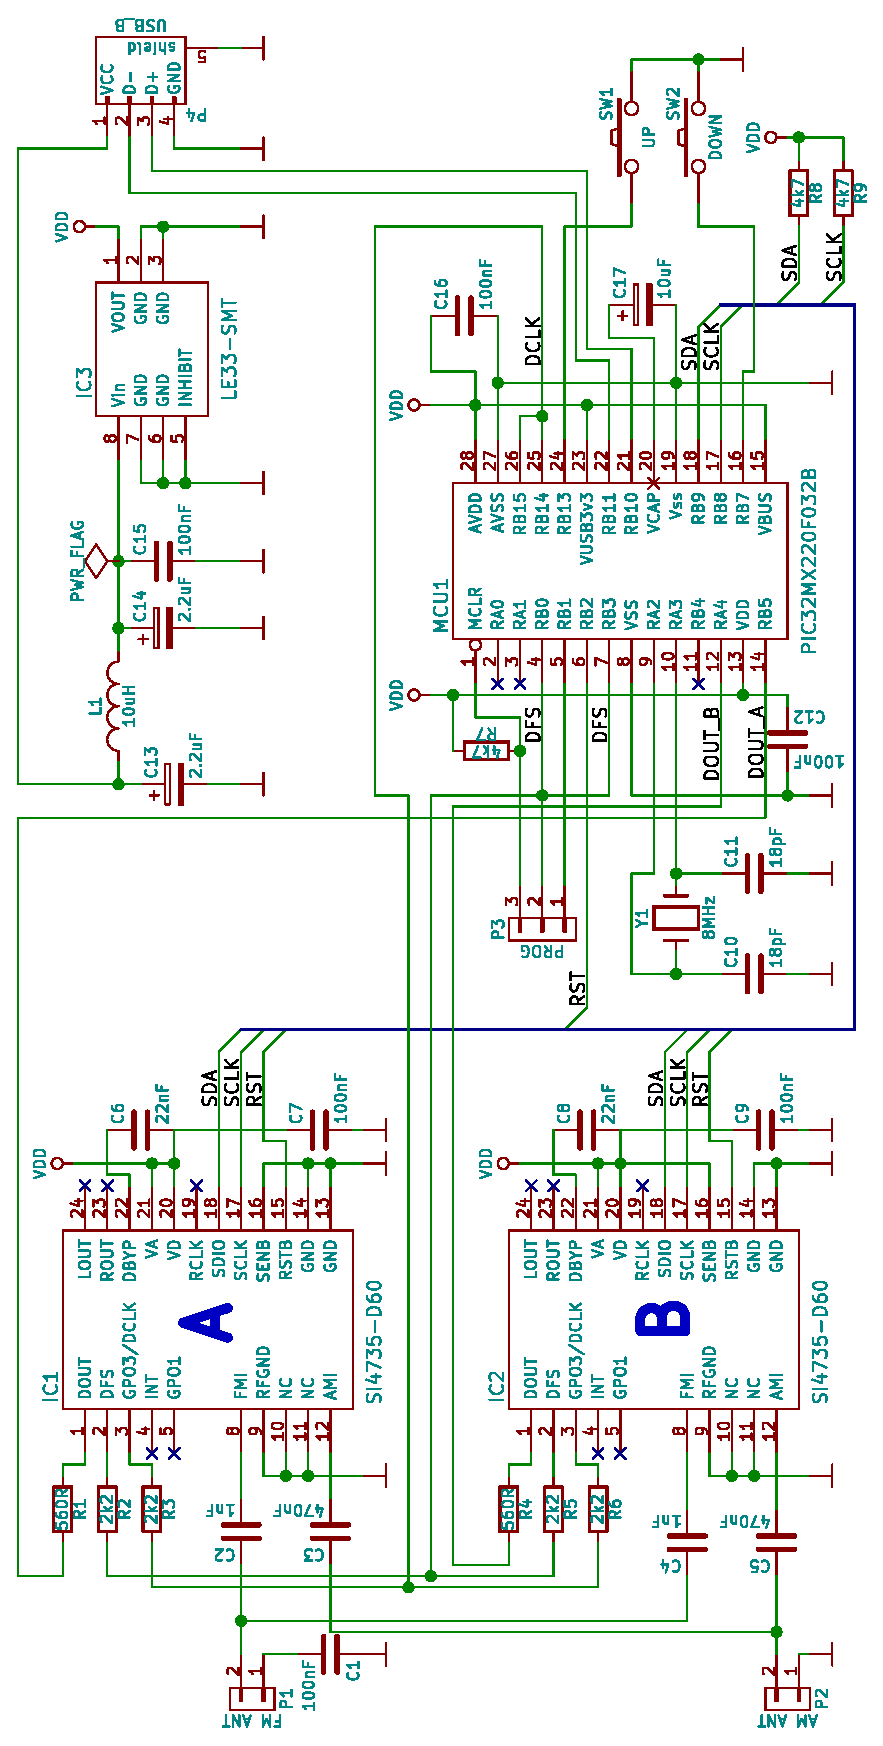
\includegraphics[scale=0.72]{figures/dfmt.eps}
\end{center}
 
\section{Rozpiska součástek}
\label{sec:ap-bom}

%\end{landscape}

\clearpage

%\InsertFigure{figures/Graf}{0.7\textwidth}{Nějaký graf}{fig:SampleGraph}

\section{Fotografie osazené desky plošných spojů}
\label{sec:ap-pcb}

\subsection*{Horní strana:}
\begin{center}
 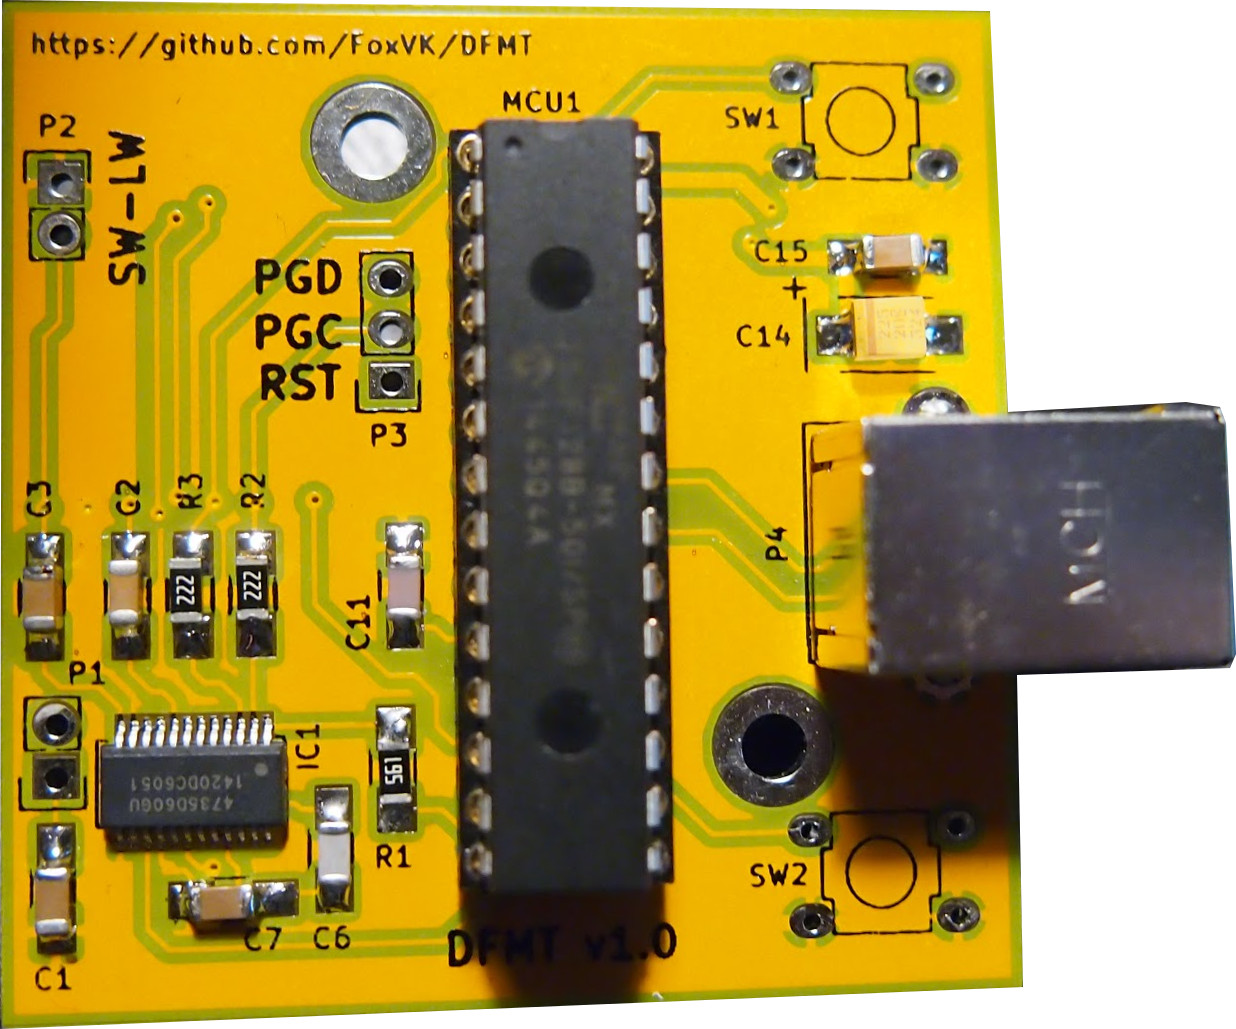
\includegraphics[scale=1]{figures/pcb-top.jpg}
\end{center}

\subsection*{Spodní strana:}
\begin{center} 
 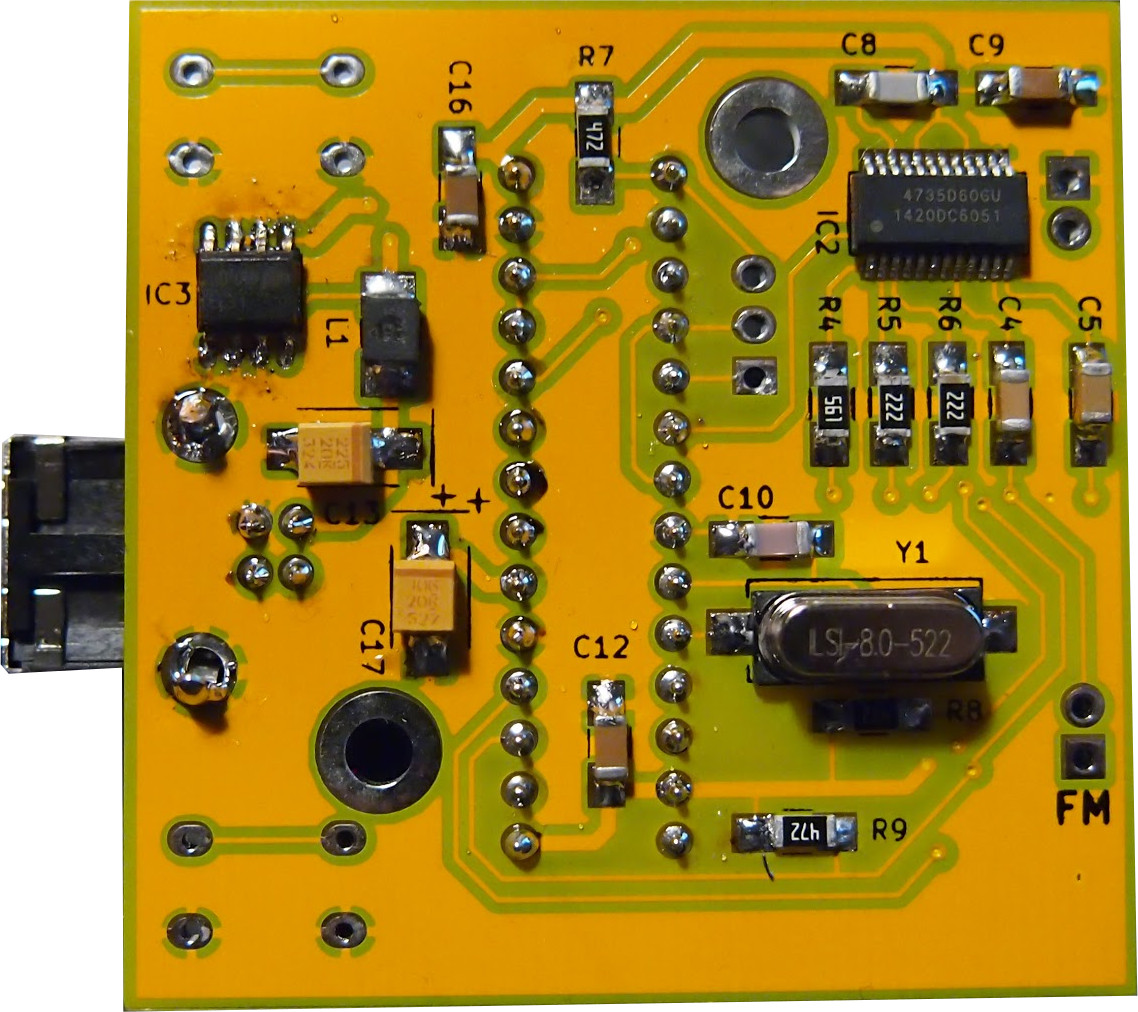
\includegraphics[scale=1]{figures/pcb-bot.jpg}
\end{center}


\end{document}
